\chapter{Унгарска осморка}

\begin{figure}[H]
  \centering
  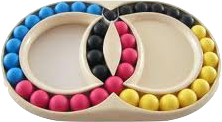
\includegraphics[width=1.0\linewidth,height=0.5\linewidth]{fig050001.png}
  \caption{„Унгарска осморка“ \\ https://www.sfu.ca/~jtmulhol/math302/images/pic-puzzle-hr.png}
\label{fig050001}
\end{figure}

Играта „Унгарска осморка“ (Фиг. \ref{fig050001}) е от групата на логическите пъзели, каквото е и кубчето на Рубик. Състои се от две пресичащи се окръжности, улеи запълнени с цветни топчета. Окръжностите се пресичат в две точки, така че две от топчетата принадлежат и на двата улея. Топчетата в улеите могат да се въртят, така че пъзелът да се разбърка. След разбъркването, целта на играта е топчетата да се подредят в първоначалното състояние. 

\section{Оформяне на интерфейса}

Макар и играта да изглежда относително елементарна, подреждането й е свързано с относителна сложност и не малко математика. Самата организация на пъзела не е особено сложна, което го прави идеален кандидат за реализация в програмна среда, каквато е Scratch. Само с помощта на тридесет и осем пулчета и четири стрелки, може да се изгради целият интерфейс на играта. Работата започва със започването на нов проект (Фиг. \ref{fig050002}).

\begin{figure}[H]
  \centering
  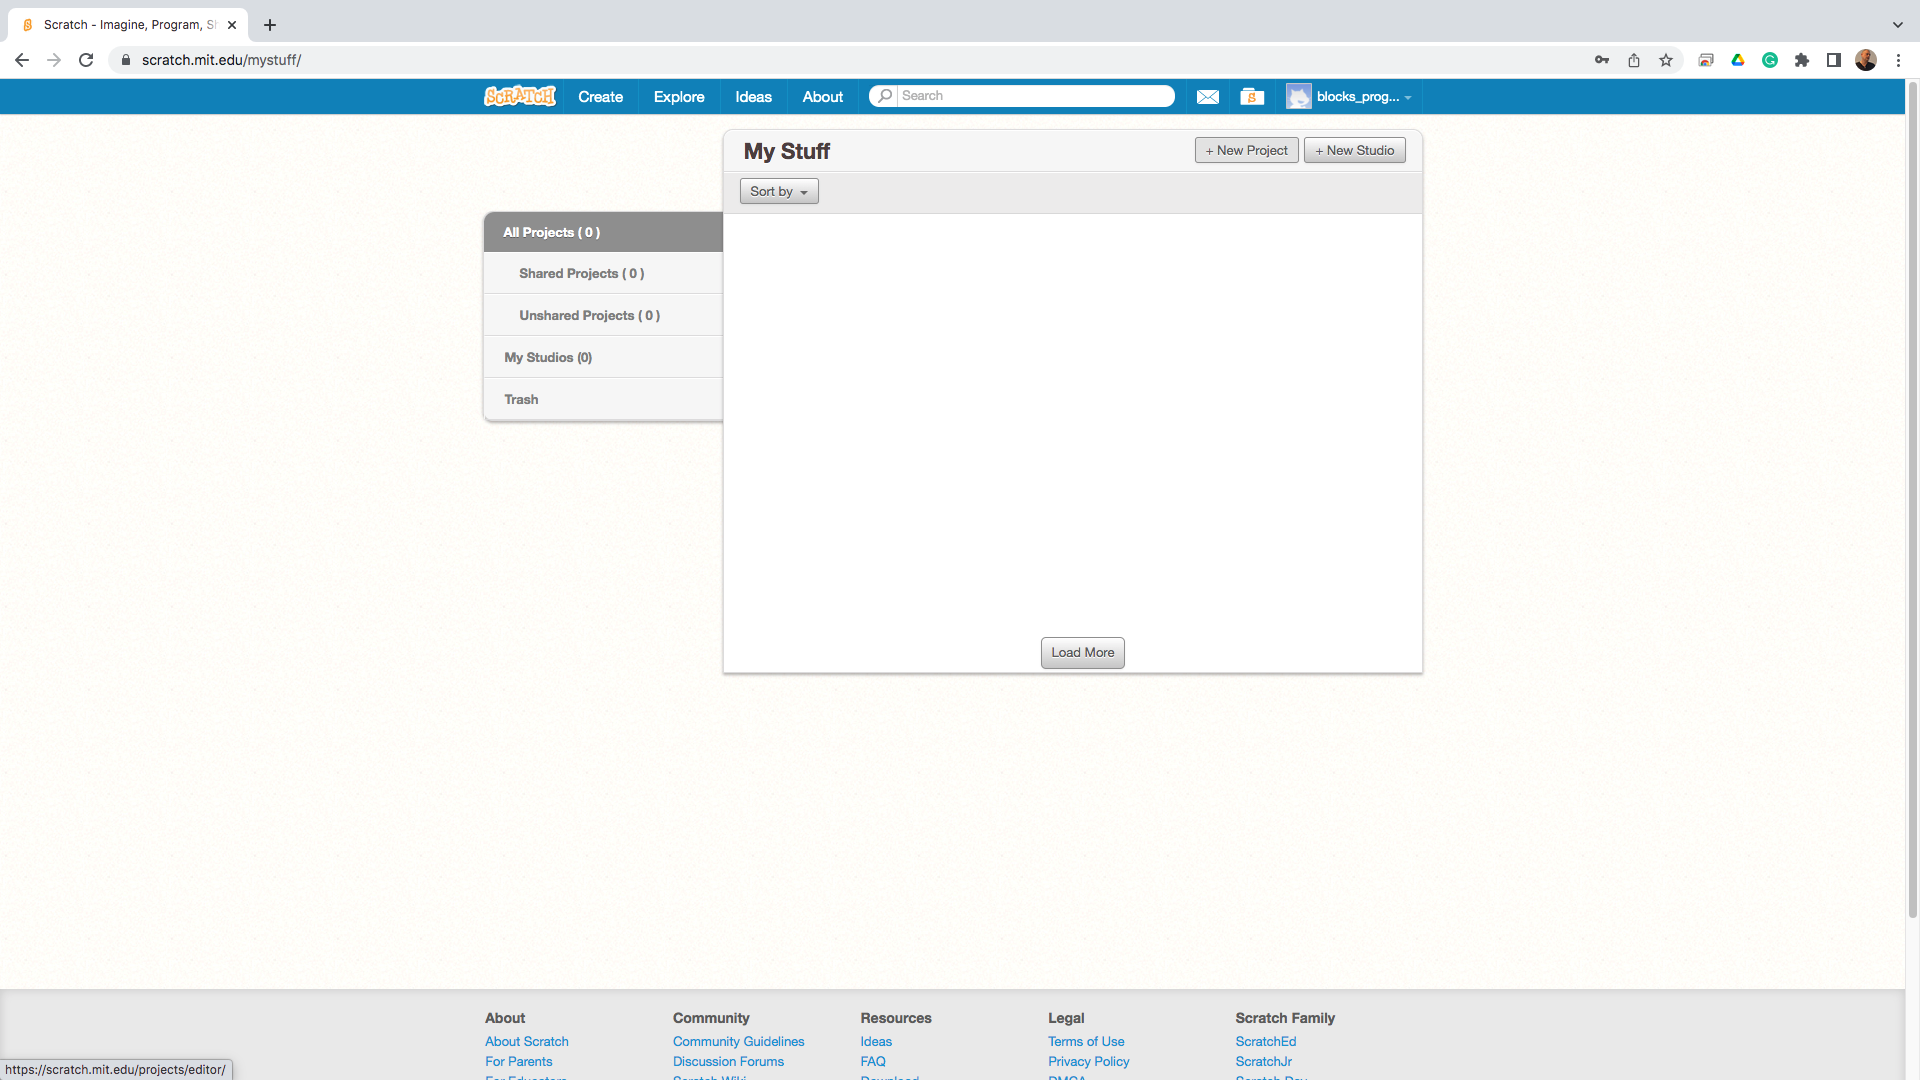
\includegraphics[width=1.0\linewidth,height=0.5\linewidth]{fig050002.png}
  \caption{Създаване на проект за „Унгарска осморка“}
\label{fig050002}
\end{figure}

Първата стъпка е да се избере име на проекта и съответно да се почисти работното пространство от спрайта на котката (Фиг. \ref{fig050003}). 

\begin{figure}[H]
  \centering
  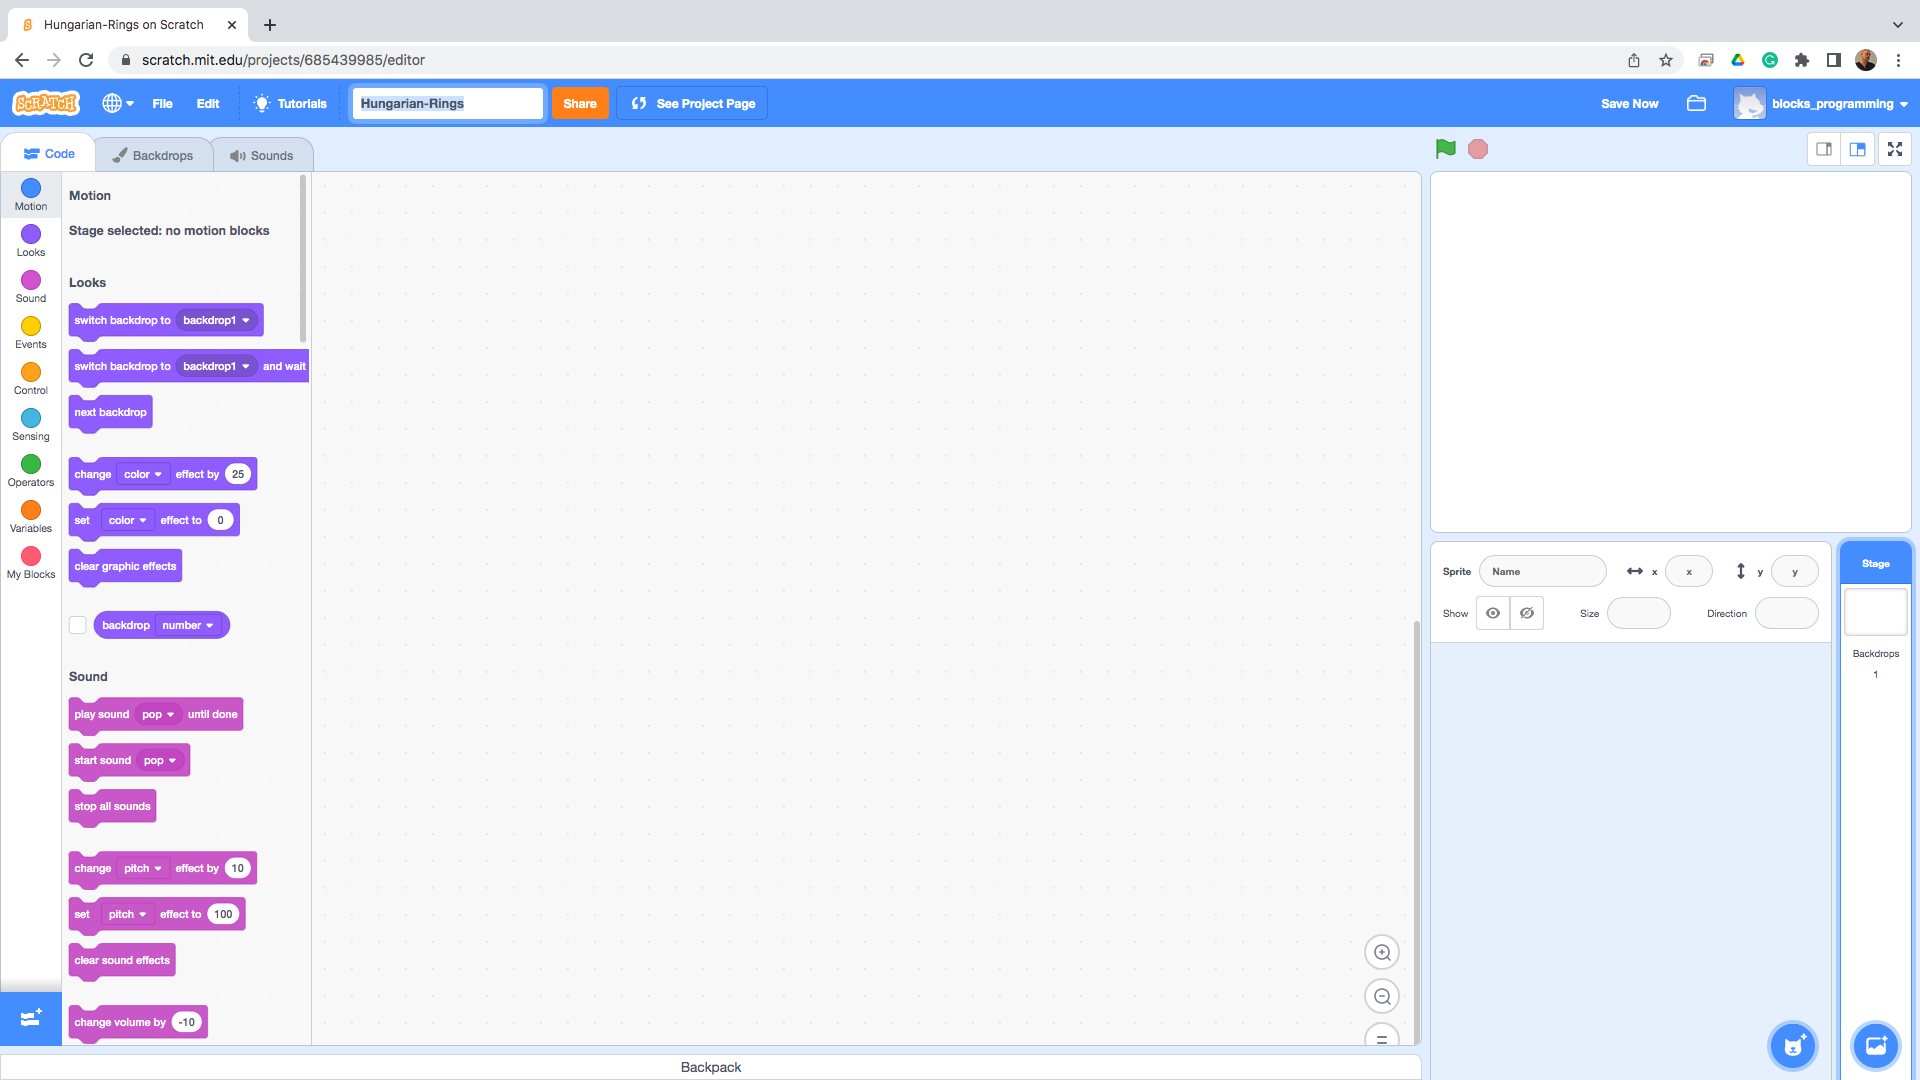
\includegraphics[width=1.0\linewidth,height=0.5\linewidth]{fig050003.png}
  \caption{Избор на име за проекта}
\label{fig050003}
\end{figure}

Разполагането на цветните топчета (в този случай пулчета) е относително трудоемка задача, тъй като трябва да се опишат две пресичащи се окръжности. Работата значително може да се улесни, ако се работи по предварително изготвена схема (Фиг. \ref{fig050004}). Схемата на пулчетата ще бъде видима само докато се подредят останалите спрайтове. В режим на игра схемата ще бъде направена невидима.

\begin{figure}[H]
  \centering
  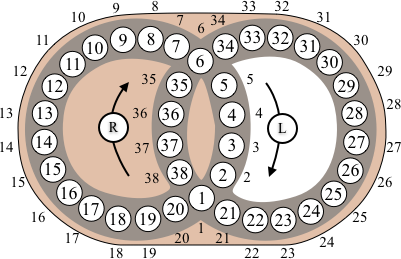
\includegraphics[width=1.0\linewidth,height=0.5\linewidth]{fig050004.png}
  \caption{Схема на играта \\ https://www.sfu.ca/~jtmulhol/math302/images/hungarianrings-labeled-nocolor.png}
\label{fig050004}
\end{figure}

Графичният файл за схемата на играта се добавя в групата от спрайтове, чрез иконката за добавяне (Фиг. \ref{fig050005}).

\begin{figure}[H]
  \centering
  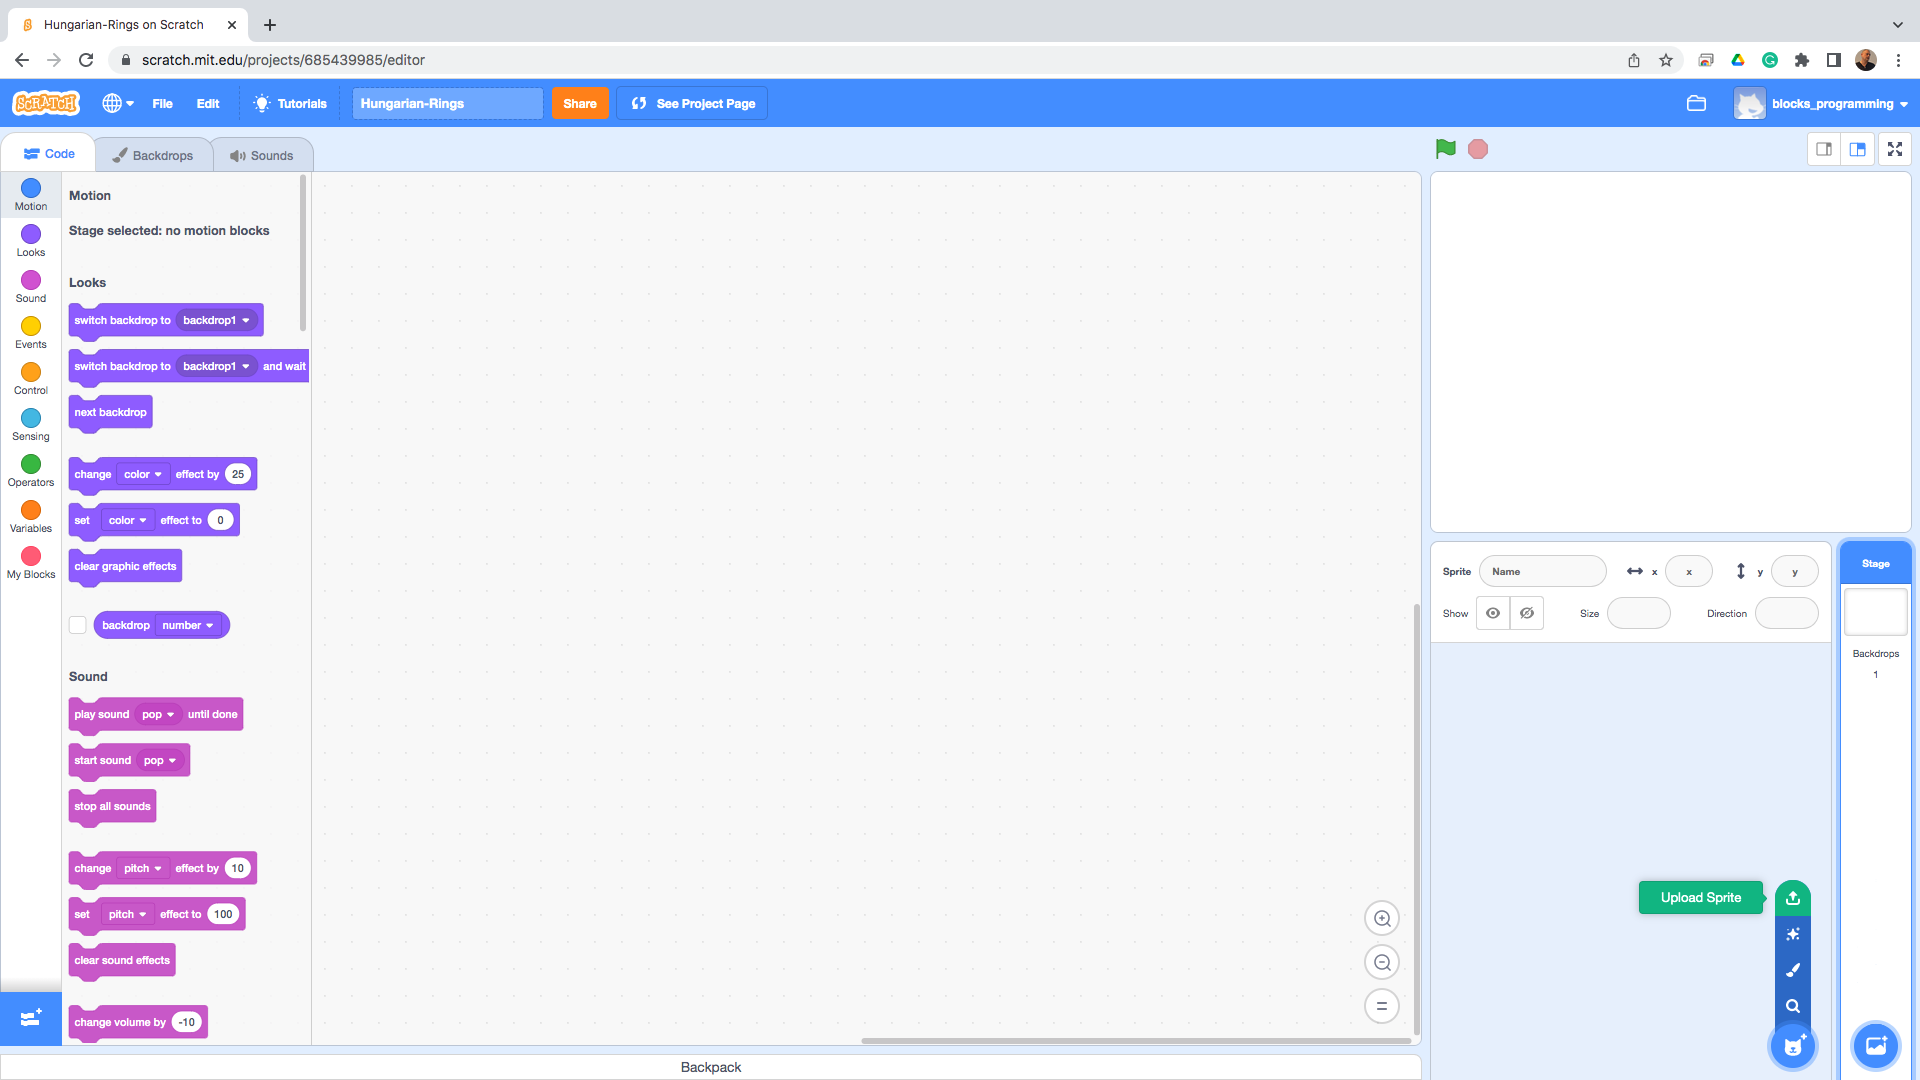
\includegraphics[width=1.0\linewidth,height=0.5\linewidth]{fig050005.png}
  \caption{Добавяне на изображението за схемата на играта}
\label{fig050005}
\end{figure}

Ново добавеният спрайт се центрира на координати x=0 и y=0 (Фиг. \ref{fig050006}), за да се постигне визуална симетрия и изображенията на предстоящите за добавяне пулчета да са в средата на визуалното пространство. 

\begin{figure}[H]
  \centering
  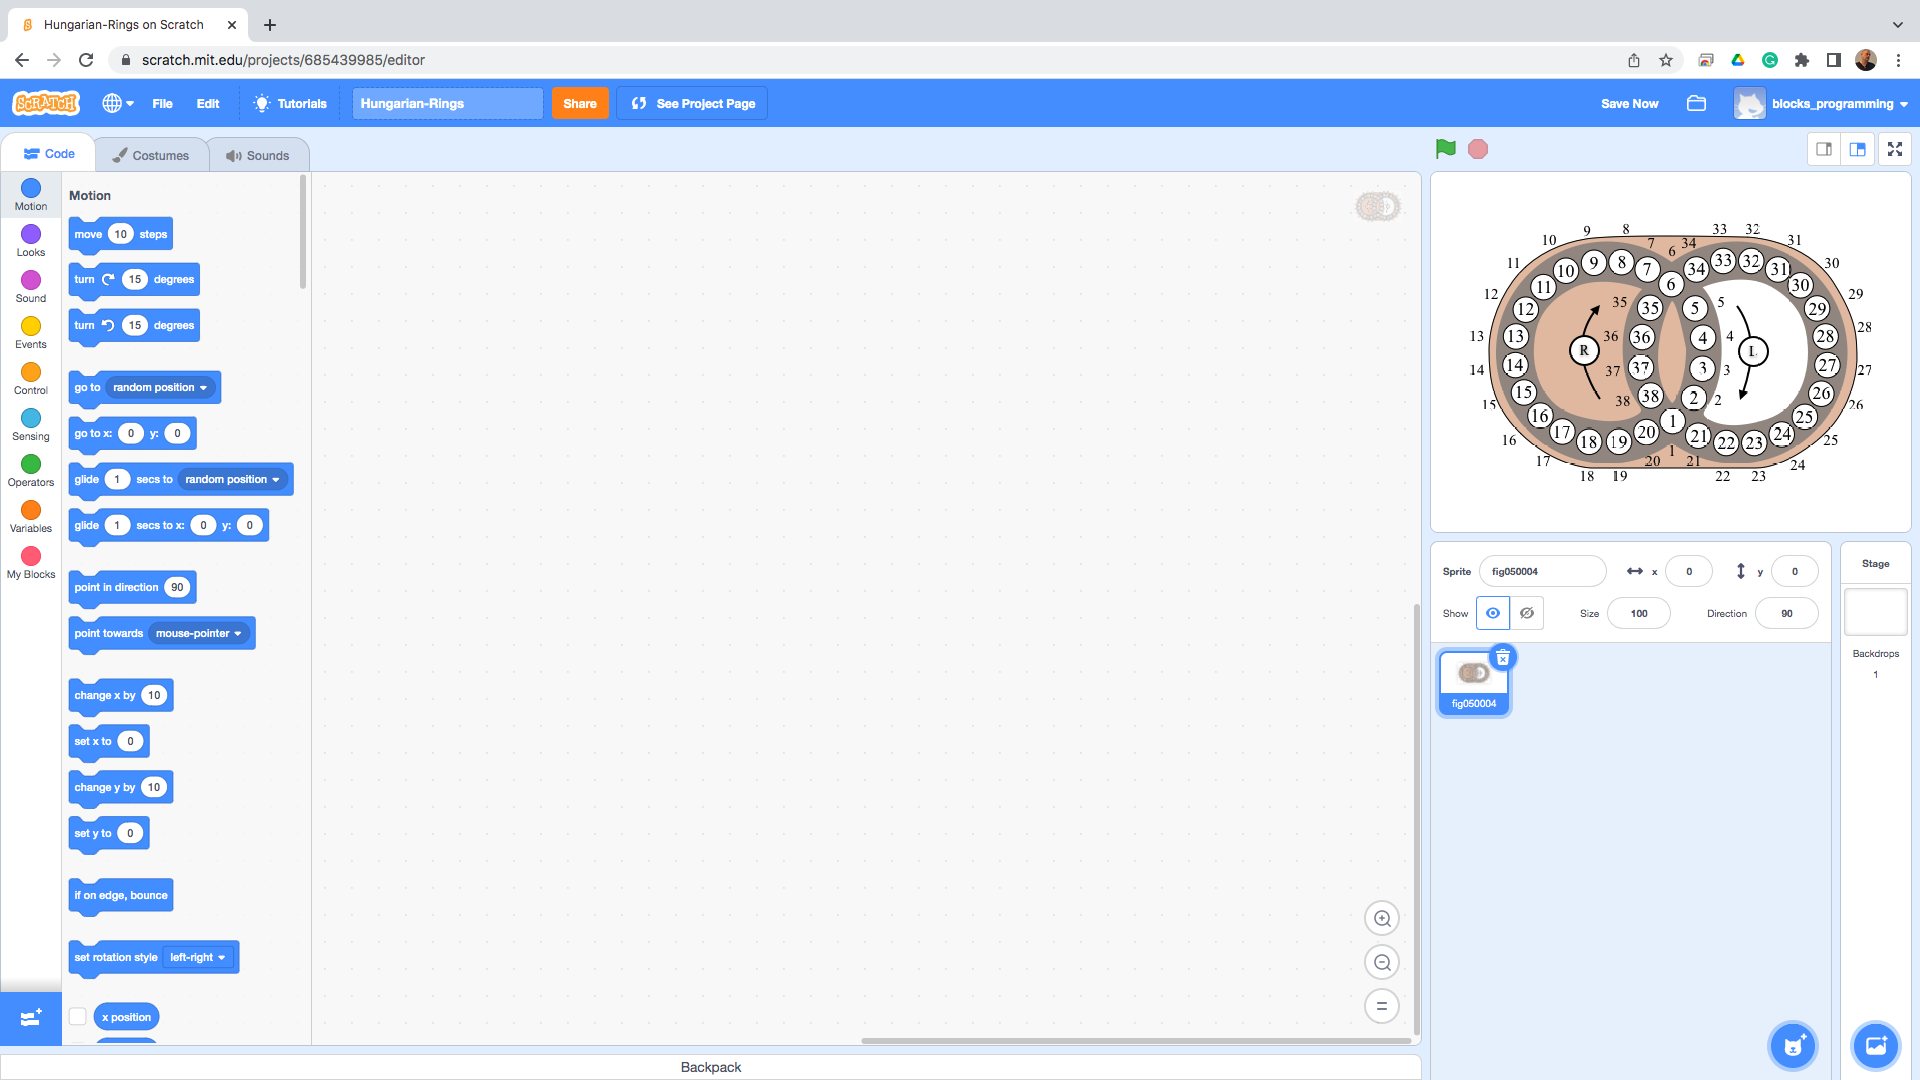
\includegraphics[width=1.0\linewidth,height=0.5\linewidth]{fig050006.png}
  \caption{Центриране на схемата}
\label{fig050006}
\end{figure}

От галерията с предварително налични спрайтове (Фиг. \ref{fig050007}) може да се избере подходящ спрайт за стрелките с които ще се предизвиква въртенето на двете окръжности.

\begin{figure}[H]
  \centering
  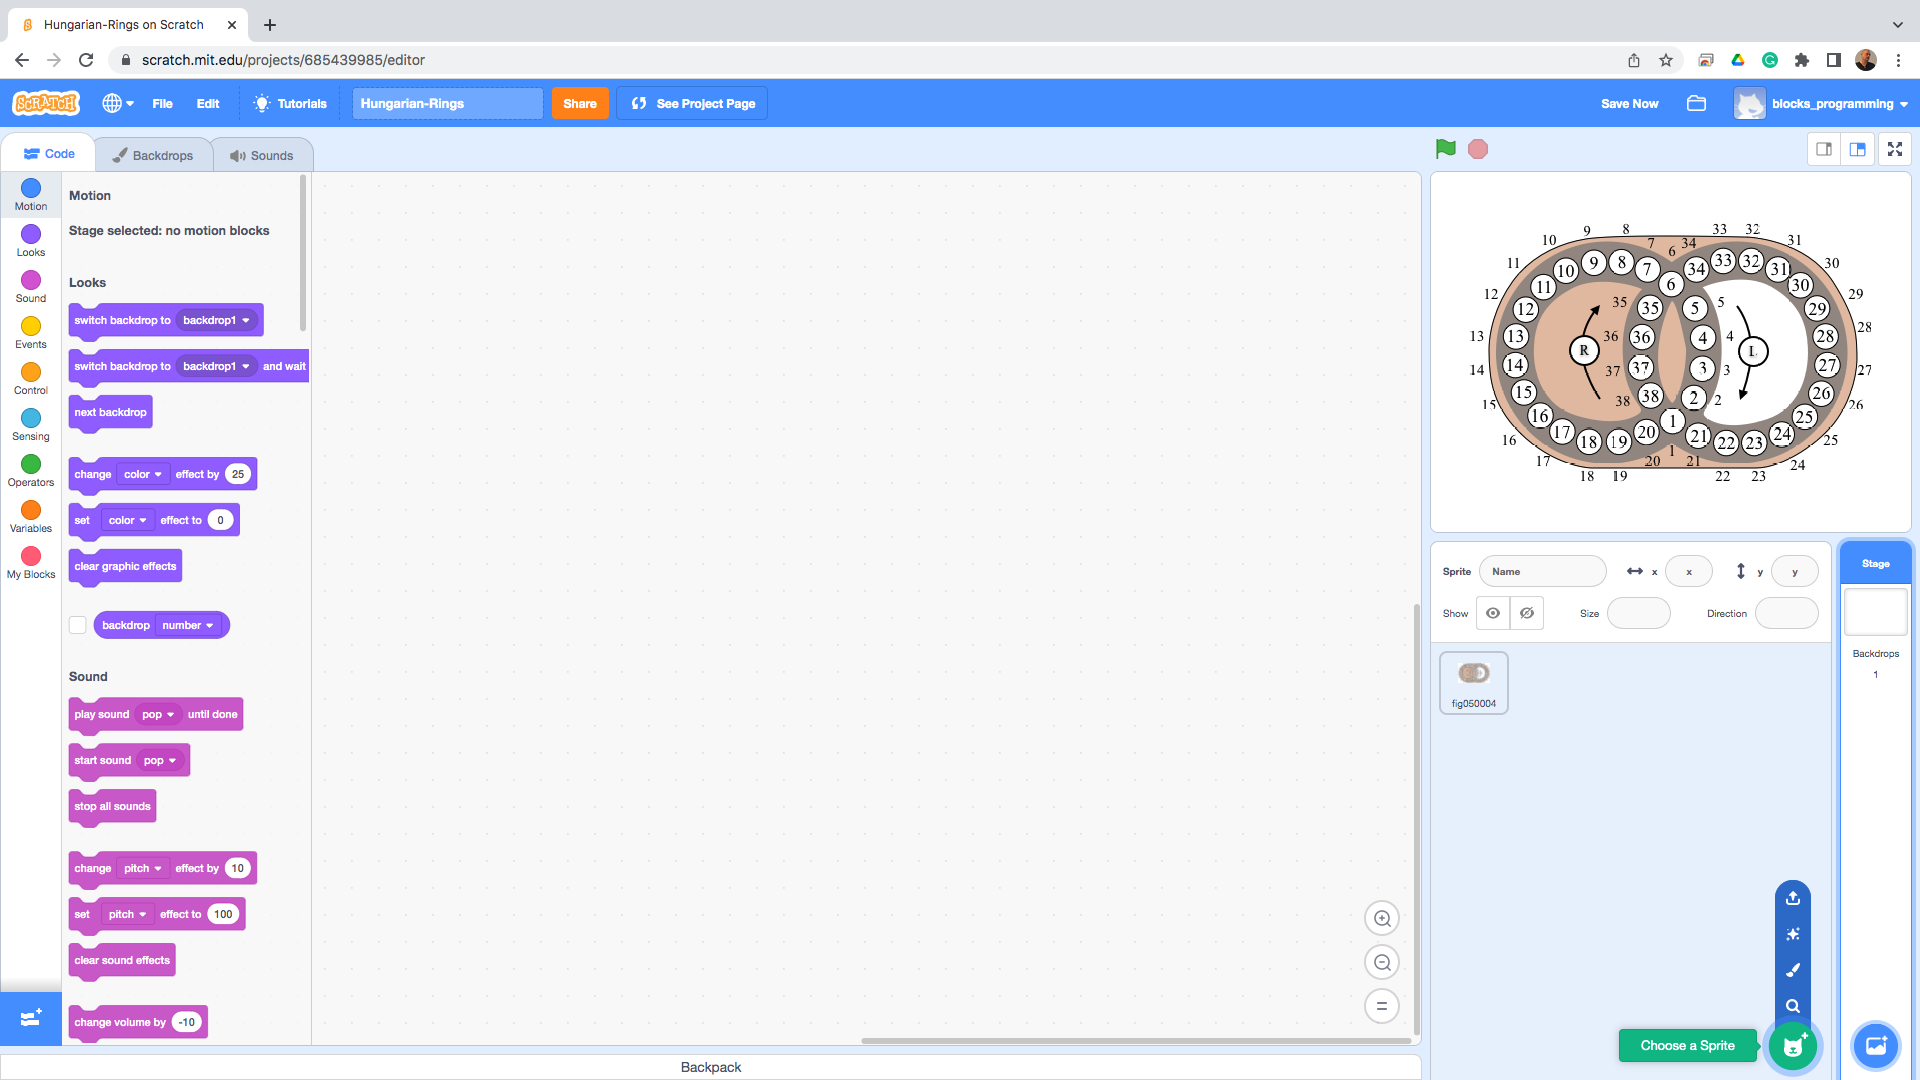
\includegraphics[width=1.0\linewidth,height=0.5\linewidth]{fig050007.png}
  \caption{Галерия с предварително налични спрайтове}
\label{fig050007}
\end{figure}

Спрайтът за стрелка има четири състояния (Фиг. \ref{fig050008}), които позволяват този спрайт да бъде използван за посоките на въртене.

\begin{figure}[H]
  \centering
  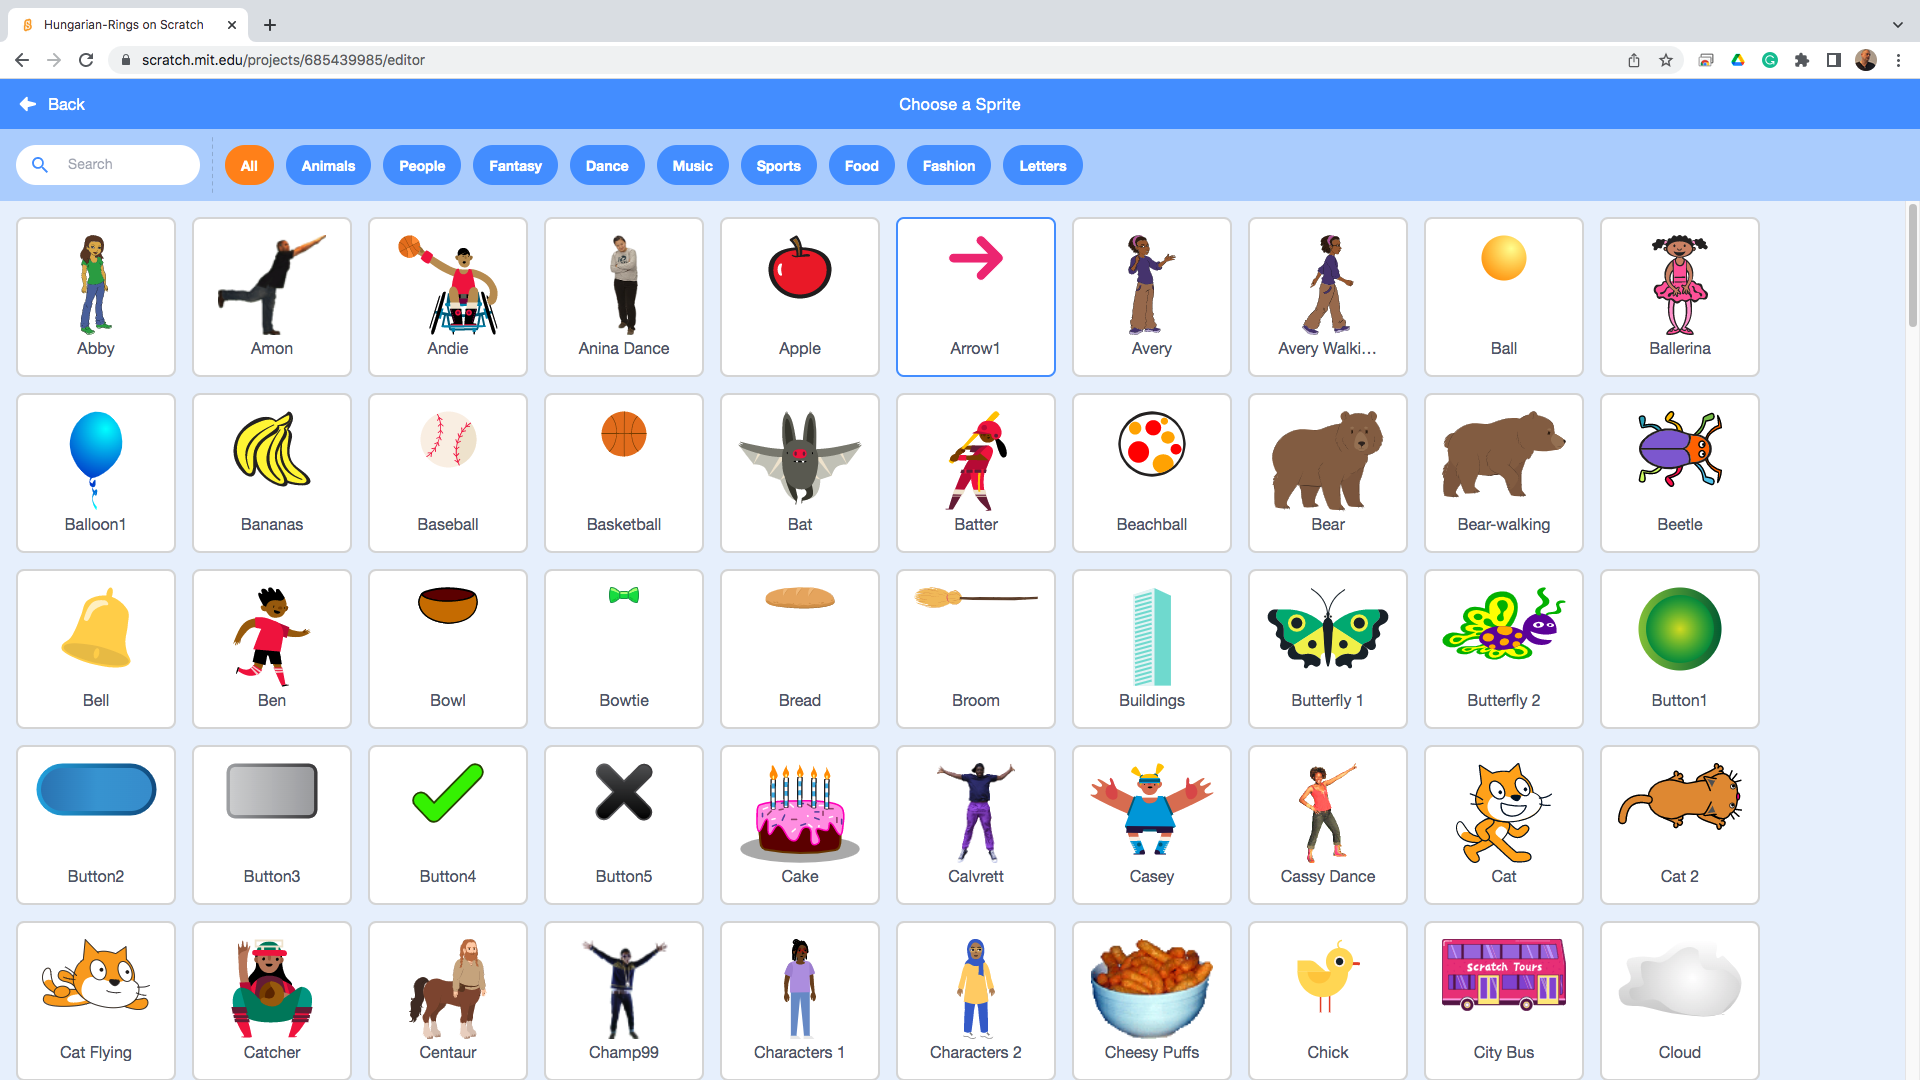
\includegraphics[width=1.0\linewidth,height=0.5\linewidth]{fig050008.png}
  \caption{Спрайт за стрелка}
\label{fig050008}
\end{figure}

Първата стрелка се разполага горе-дясно (Фиг. \ref{fig050009}), като тя ще служи за завъртане на десният ринг в посока по часовниковата стрелка.

\begin{figure}[H]
  \centering
  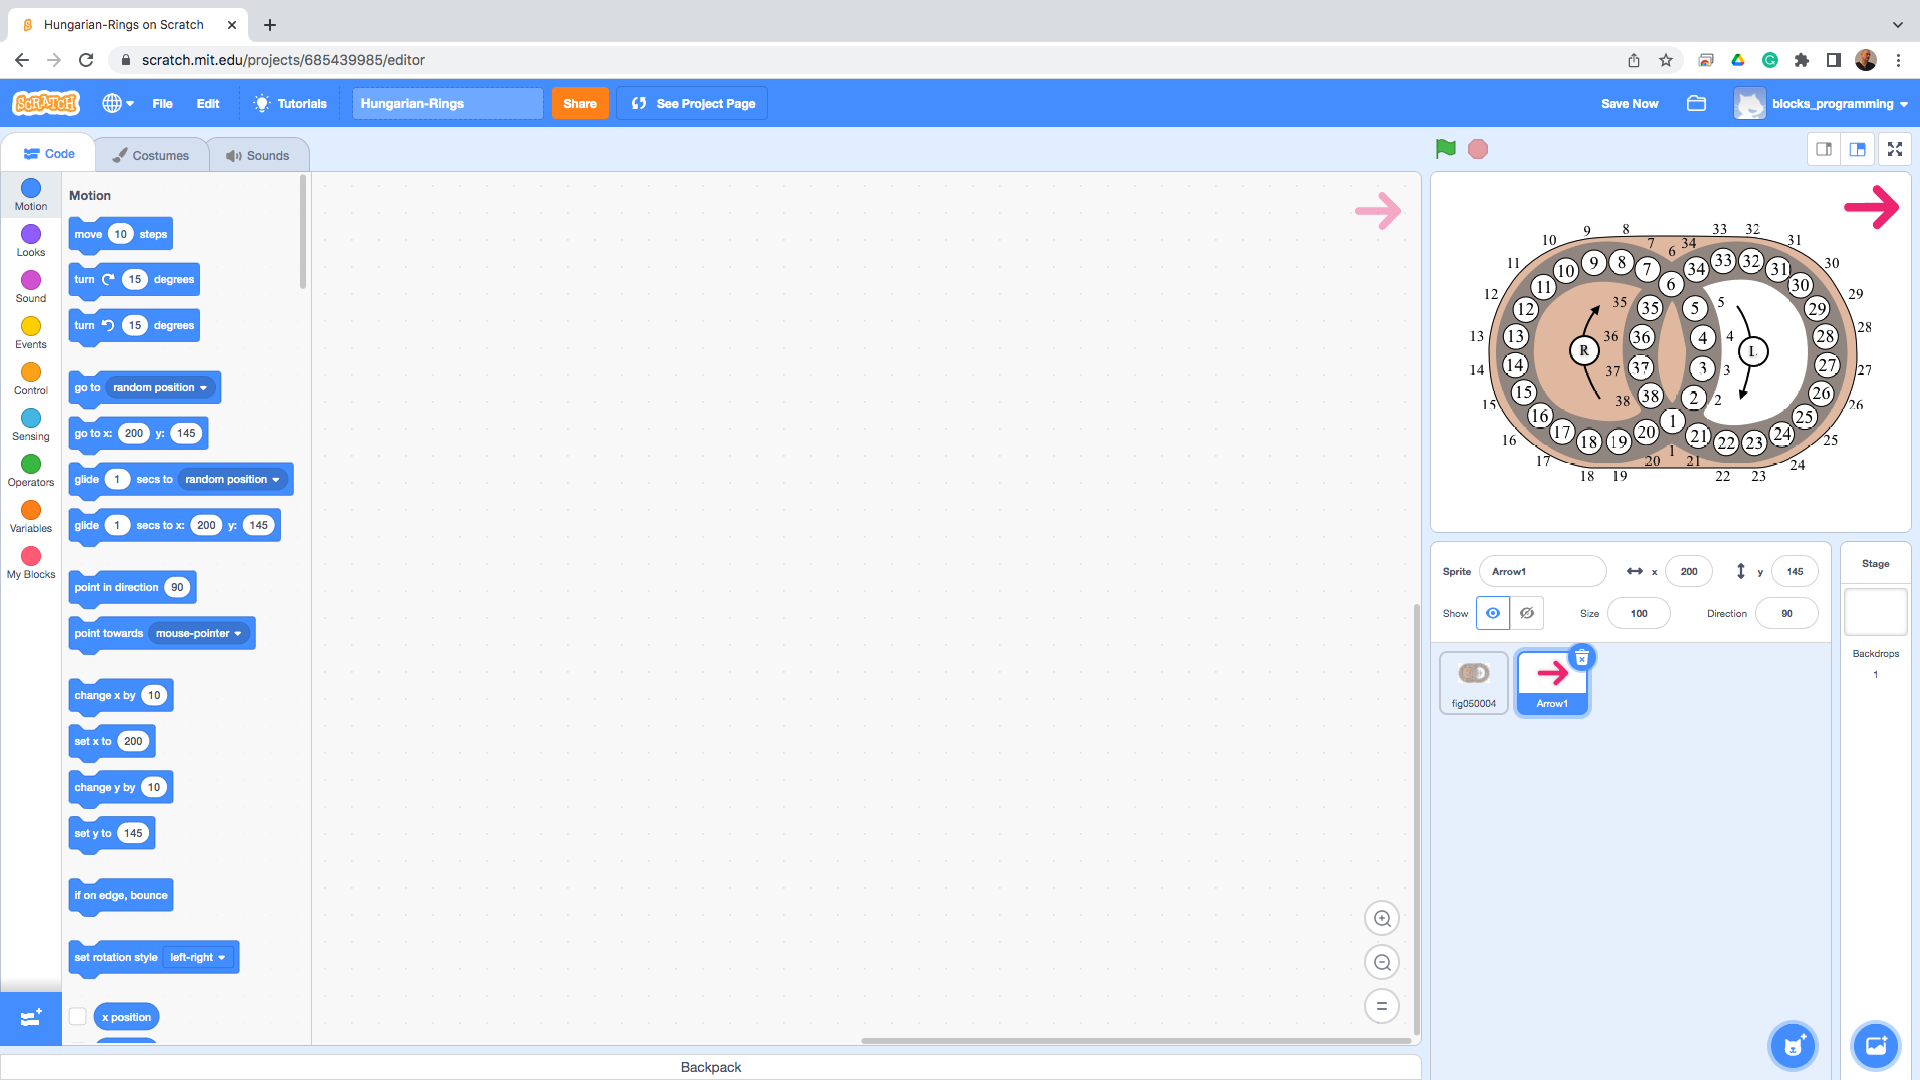
\includegraphics[width=1.0\linewidth,height=0.5\linewidth]{fig050009.png}
  \caption{Стрелка за завъртане на десния ринг по часовниковата стрелка}
\label{fig050009}
\end{figure}

Втората стрелка се разполага долу-дясно (Фиг. \ref{fig050010}), като тя ще служи за завъртане на десния ринг в посока обратна на часовниковата стрелка.

\begin{figure}[H]
  \centering
  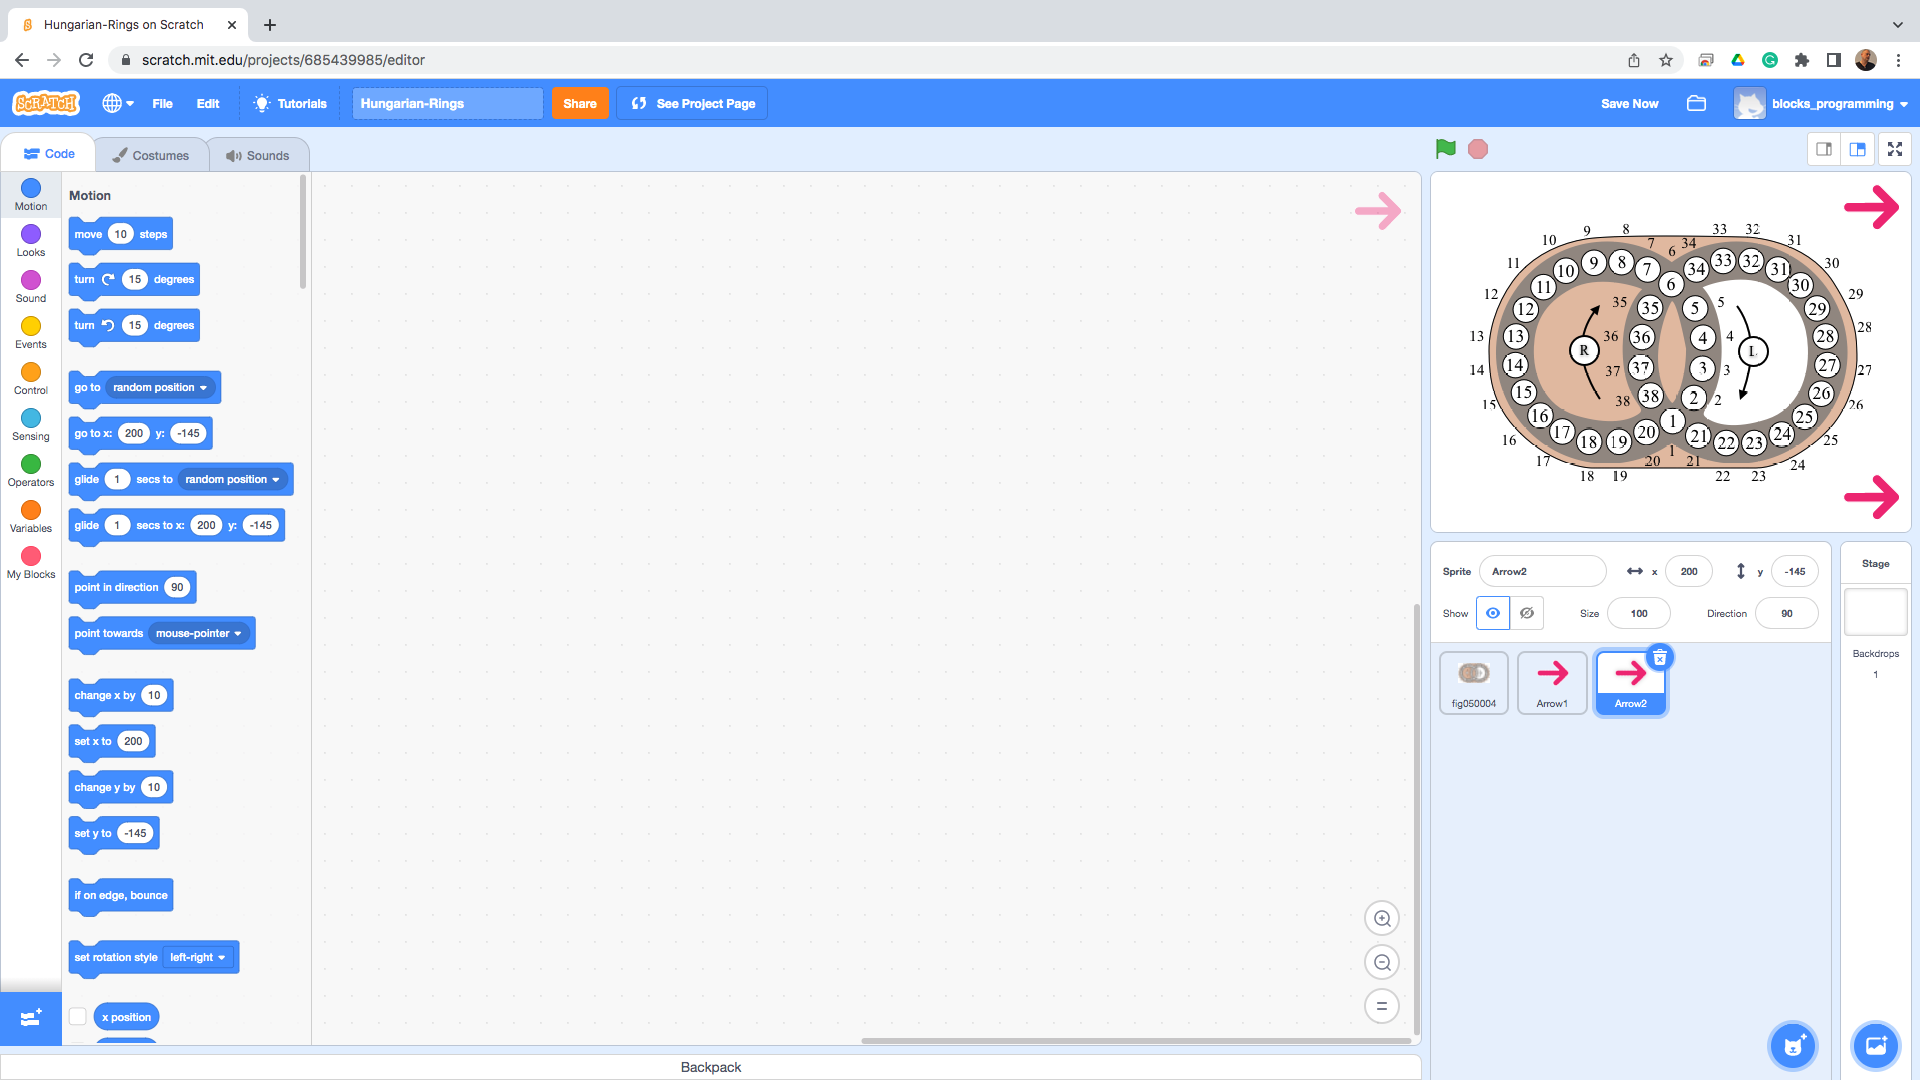
\includegraphics[width=1.0\linewidth,height=0.5\linewidth]{fig050010.png}
  \caption{Стрелка за завъртане на десния ринг обратно на часовниковата стрелка}
\label{fig050010}
\end{figure}

Третата стрелка се разполага долу-ляво, като се избира за активен вторият кадър в спрайта, така че стрелката да сочи на ляво (Фиг. \ref{fig050011}).

\begin{figure}[H]
  \centering
  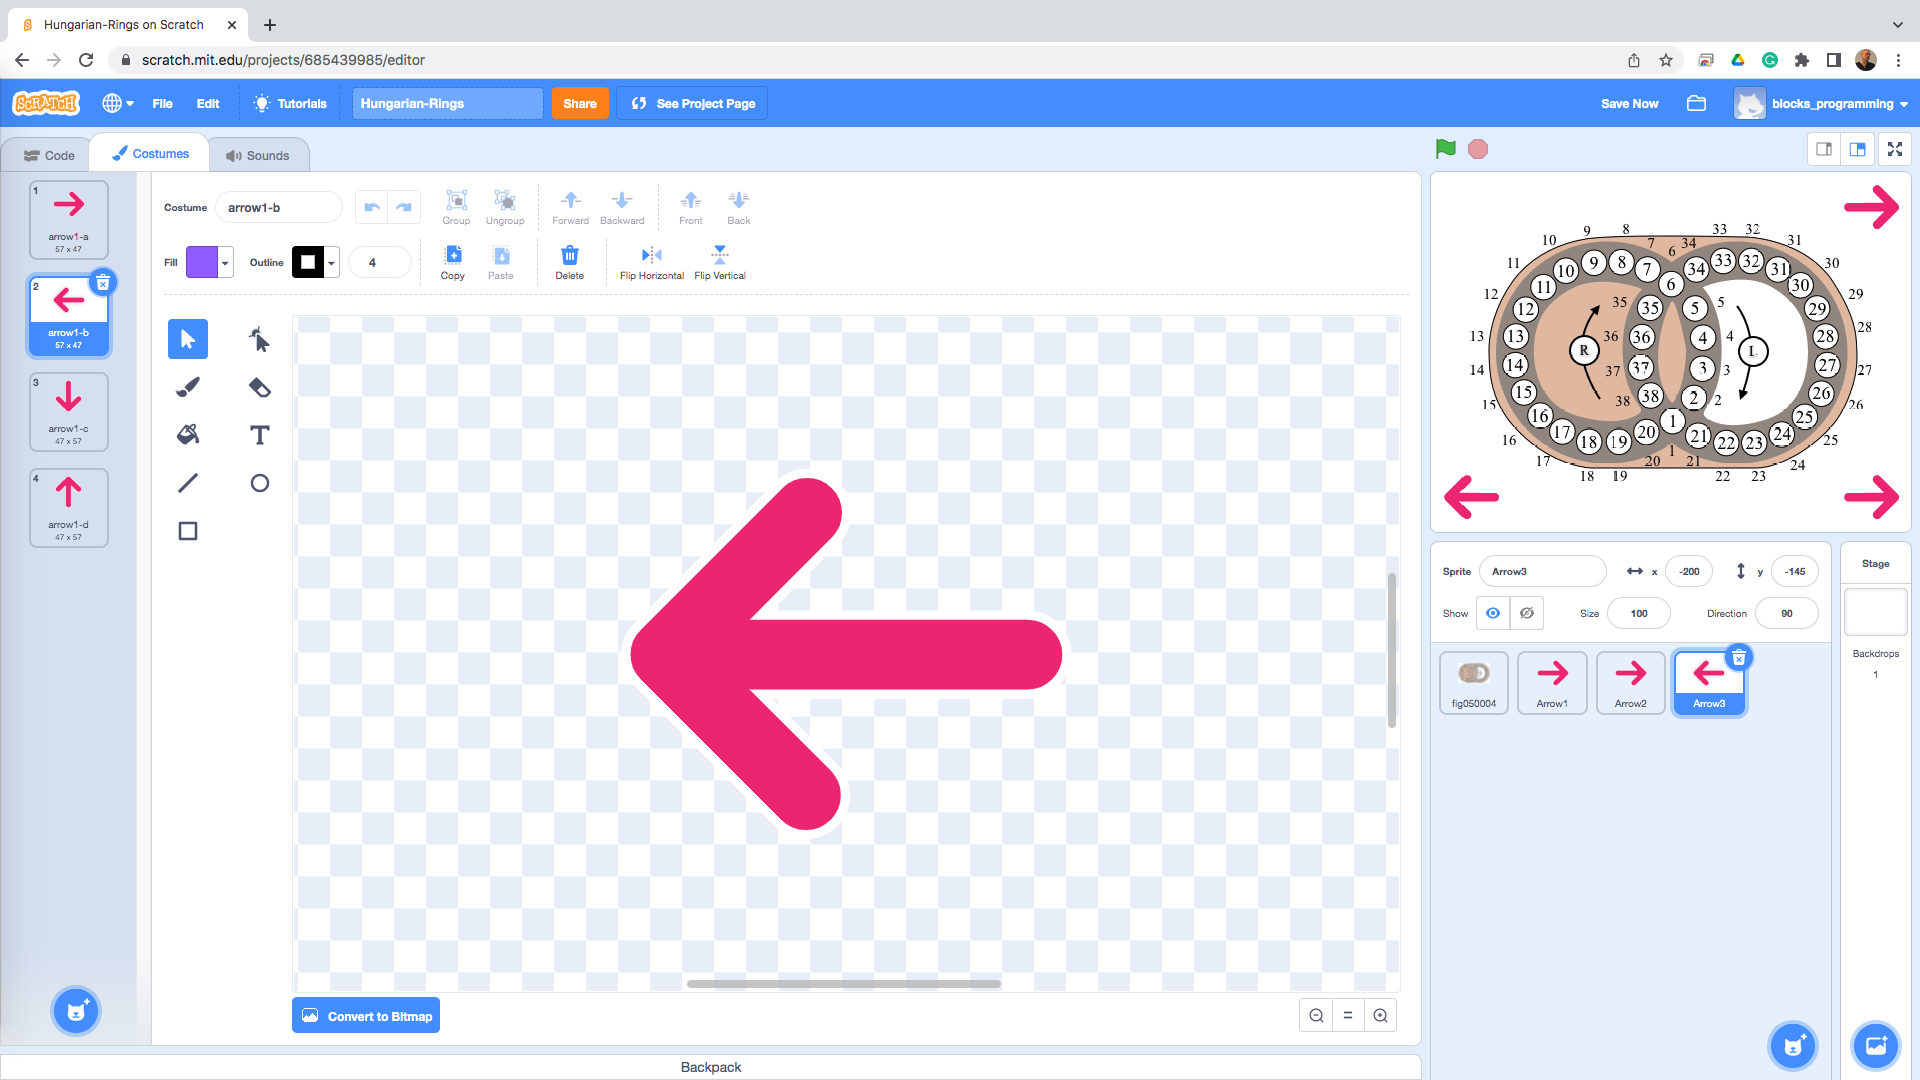
\includegraphics[width=1.0\linewidth,height=0.5\linewidth]{fig050011.png}
  \caption{Стрелка за завъртане на левия ринг по часовниковата стрелка}
\label{fig050011}
\end{figure}

Четвъртата стрелка се разполага горе-ляво (Фиг. \ref{fig050012}), като нейната задача е да води до завъртане на левия ринг по посока обратна на часовниковата стрелка.

\begin{figure}[H]
  \centering
  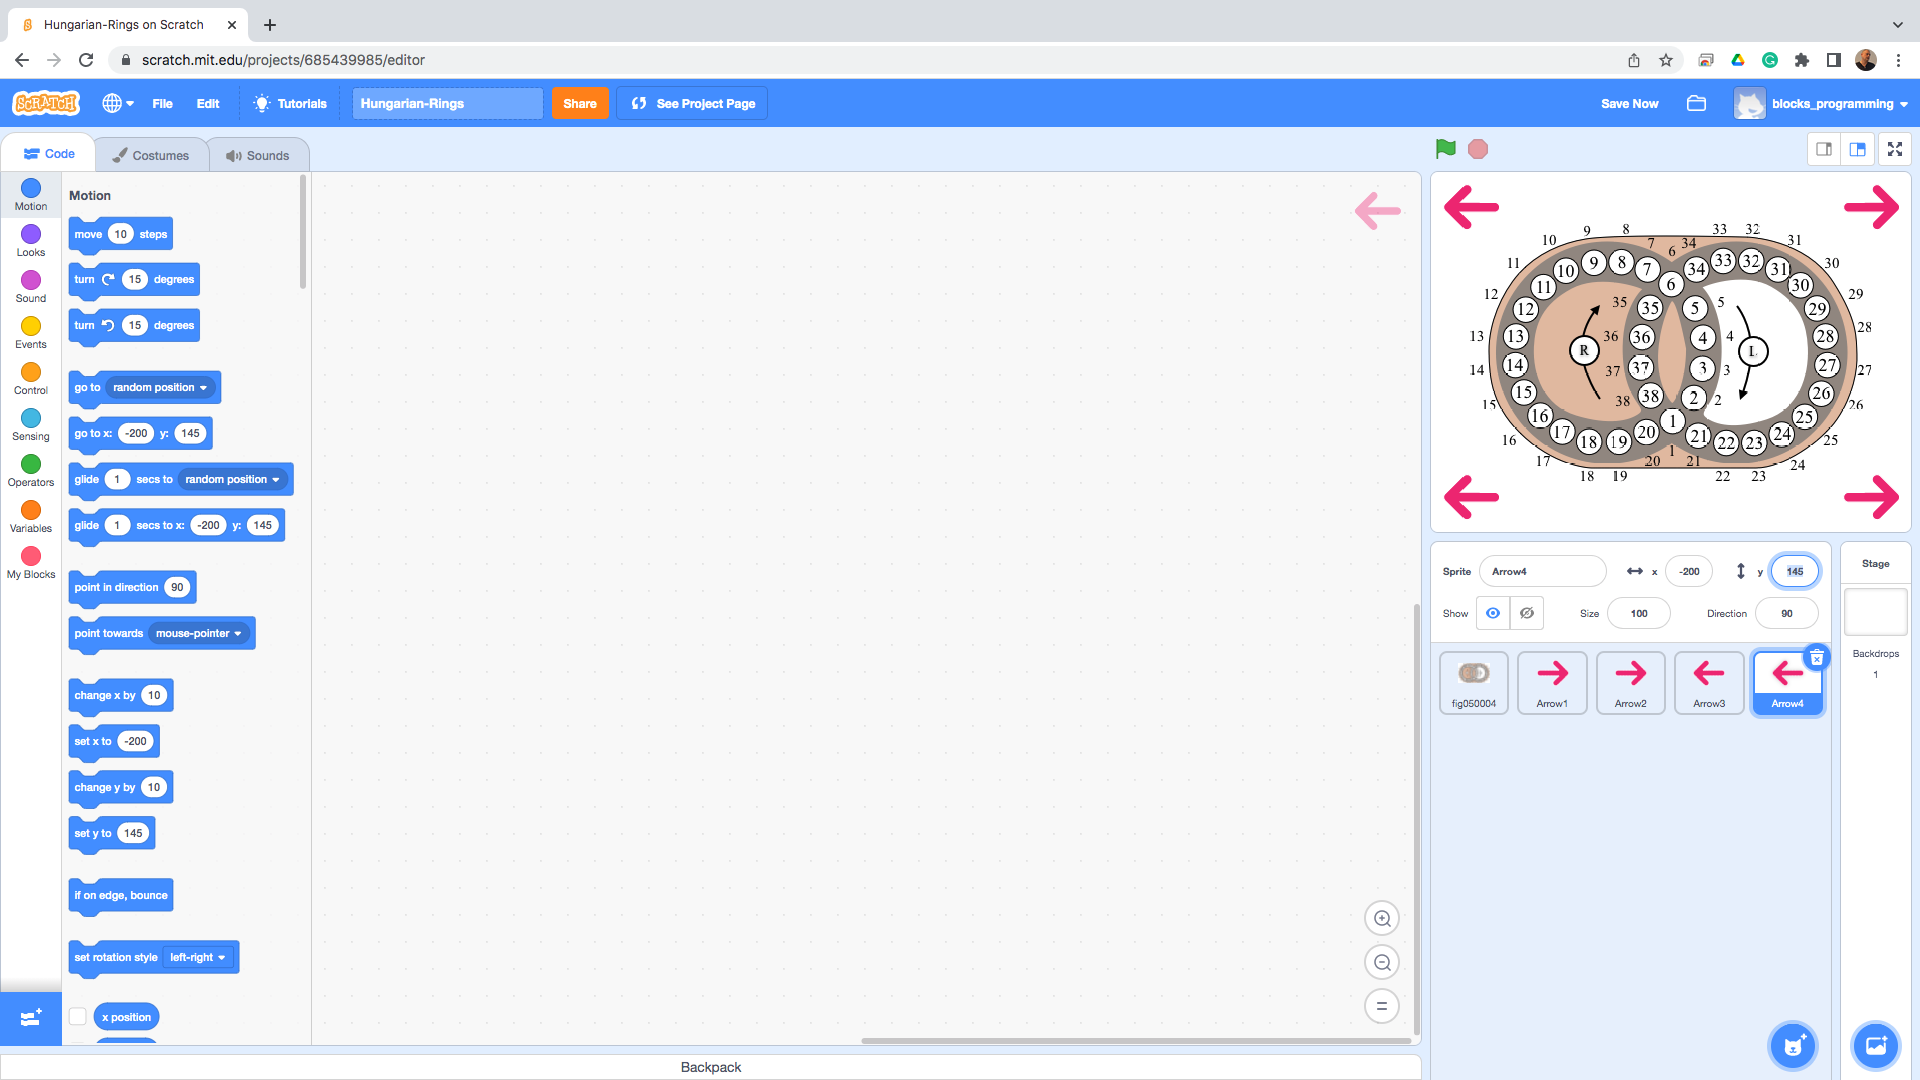
\includegraphics[width=1.0\linewidth,height=0.5\linewidth]{fig050012.png}
  \caption{Стрелка за завъртане на левия ринг обратно на часовниковата стрелка}
\label{fig050012}
\end{figure}

Една от възможностите за онагледяване на топчетата от оригиналната игра е чрез спрайта за топка (Фиг. \ref{fig050013}). Този спрайт позволява топката да бъде визуализирана в няколко различни цвята, което идеално пасва на необходимостта да се визуализират четири различни по цвят топчета.

\begin{figure}[H]
  \centering
  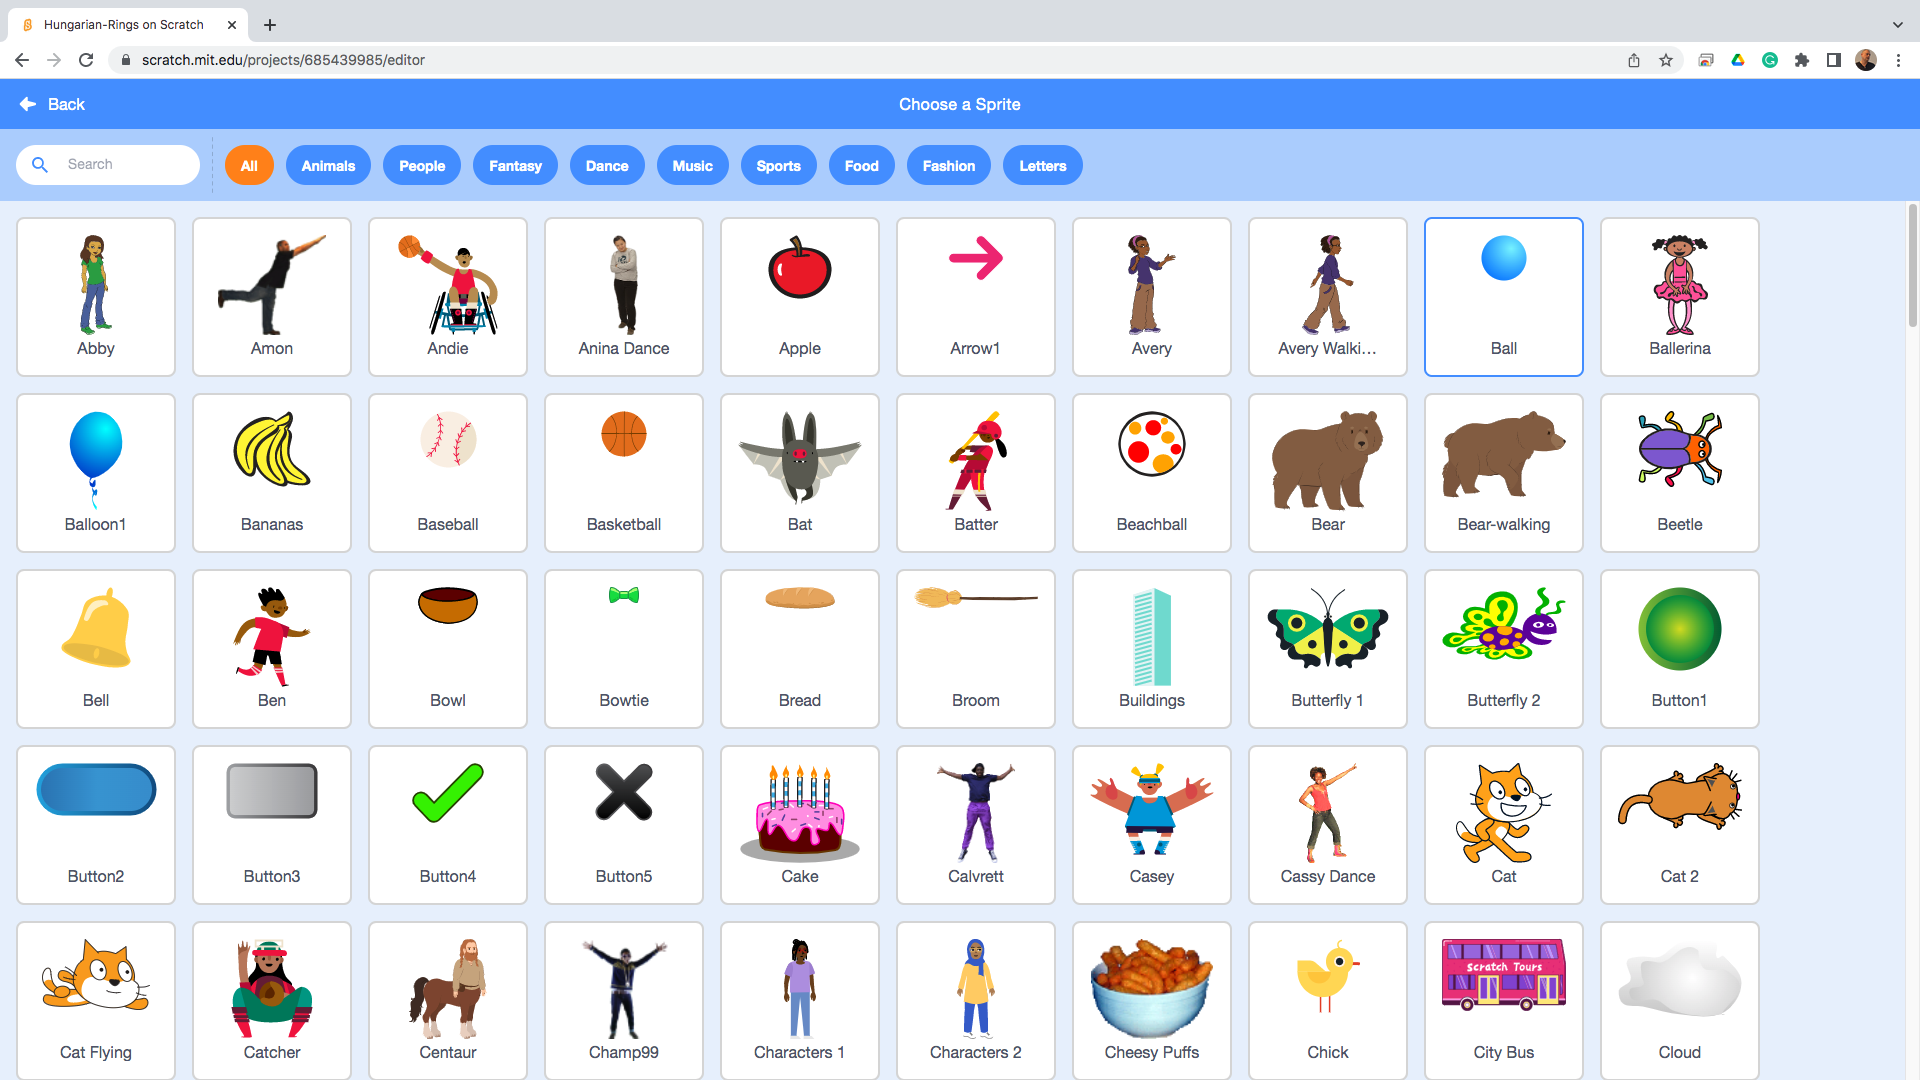
\includegraphics[width=1.0\linewidth,height=0.5\linewidth]{fig050013.png}
  \caption{Избор на спрайт за точетата}
\label{fig050013}
\end{figure}

Първото поставено пулче отива на позицията означена с номер едно на вече включената схема. За да се наслагват успешно различните спрайтове е необходимо спрайта на схемата да бъде изпратен най-отзад в Z-буфера, така че всички други спрайтове да се визуализират пред него. 

Пулчето се смалява (в случая до 55) и след това с помощта на мишката се нагласява да попадне точно върху пространството, маркирано с единица (Фиг. \ref{fig050014}). 

\begin{figure}[H]
  \centering
  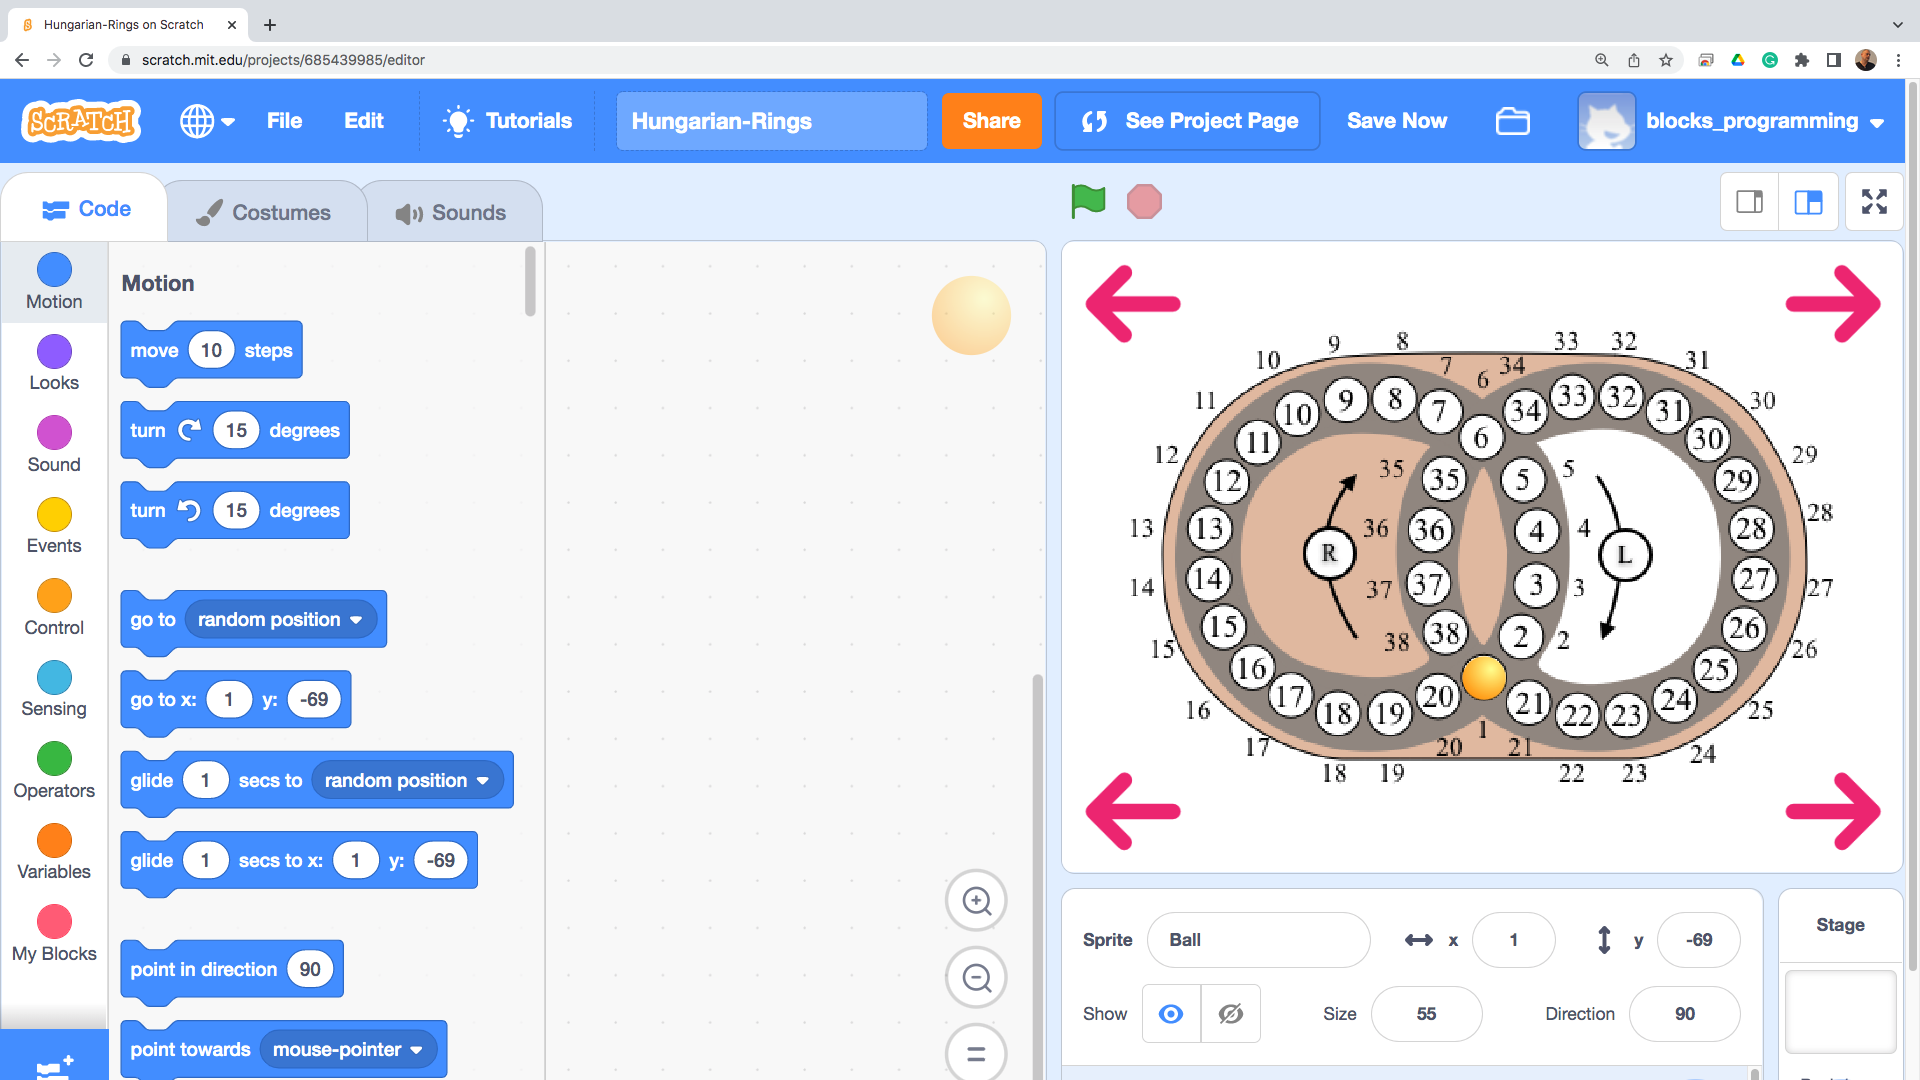
\includegraphics[width=1.0\linewidth,height=0.5\linewidth]{fig050014.png}
  \caption{Оразмеряване и позициониране на първото пулче}
\label{fig050014}
\end{figure}

\section{Структури от данни}

Когато игата започне (Фиг. \ref{fig050015}), състоянието на игралното поле ще се отразява в списъчна структура. Числата от едно до четири ще отразяват какъв цвят топче трябва да бъде визуализирано на позицията със съответен номер.

\begin{figure}[H]
  \centering
  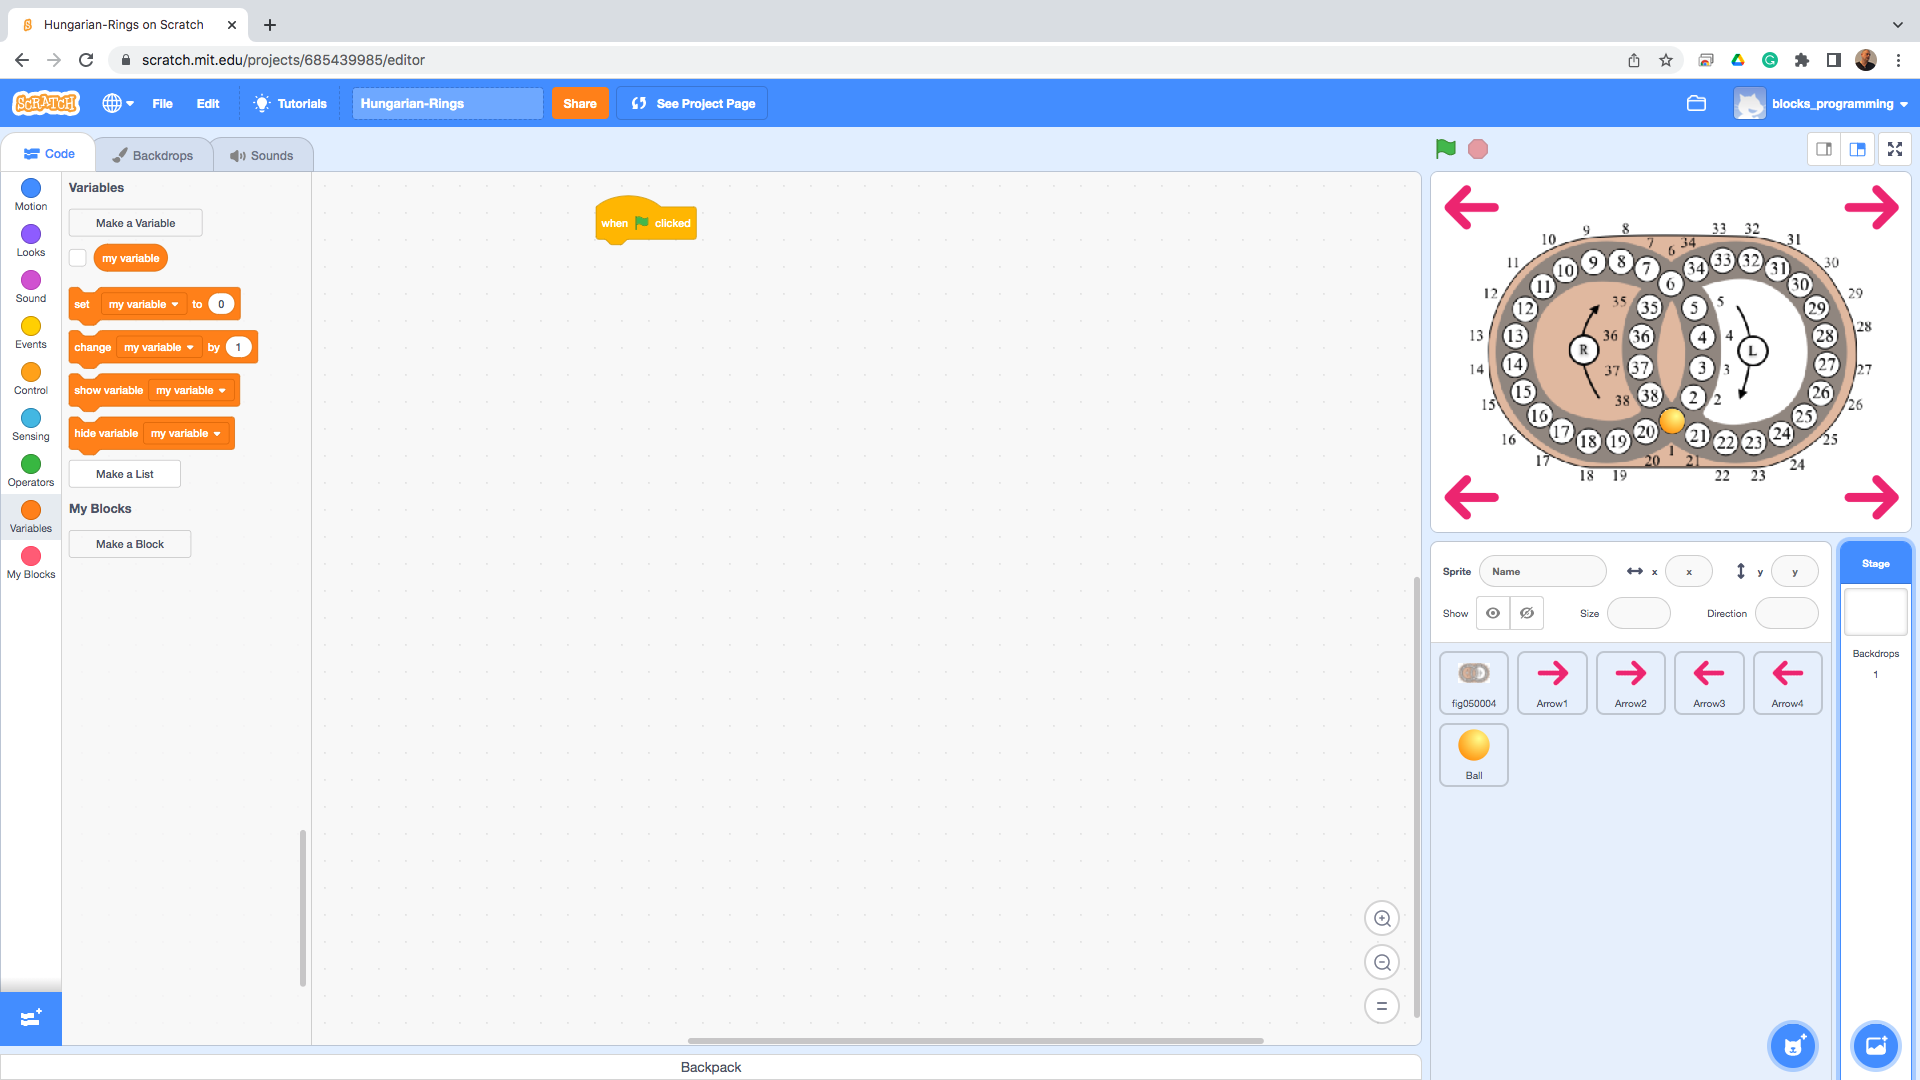
\includegraphics[width=1.0\linewidth,height=0.5\linewidth]{fig050015.png}
  \caption{Начало на играта в програмното поле на сцената}
\label{fig050015}
\end{figure}

За тази цел се създава списък „state“ и в него ще бъдат записани числата, определящи цветовете на пулчетата. 

\begin{figure}[H]
  \centering
  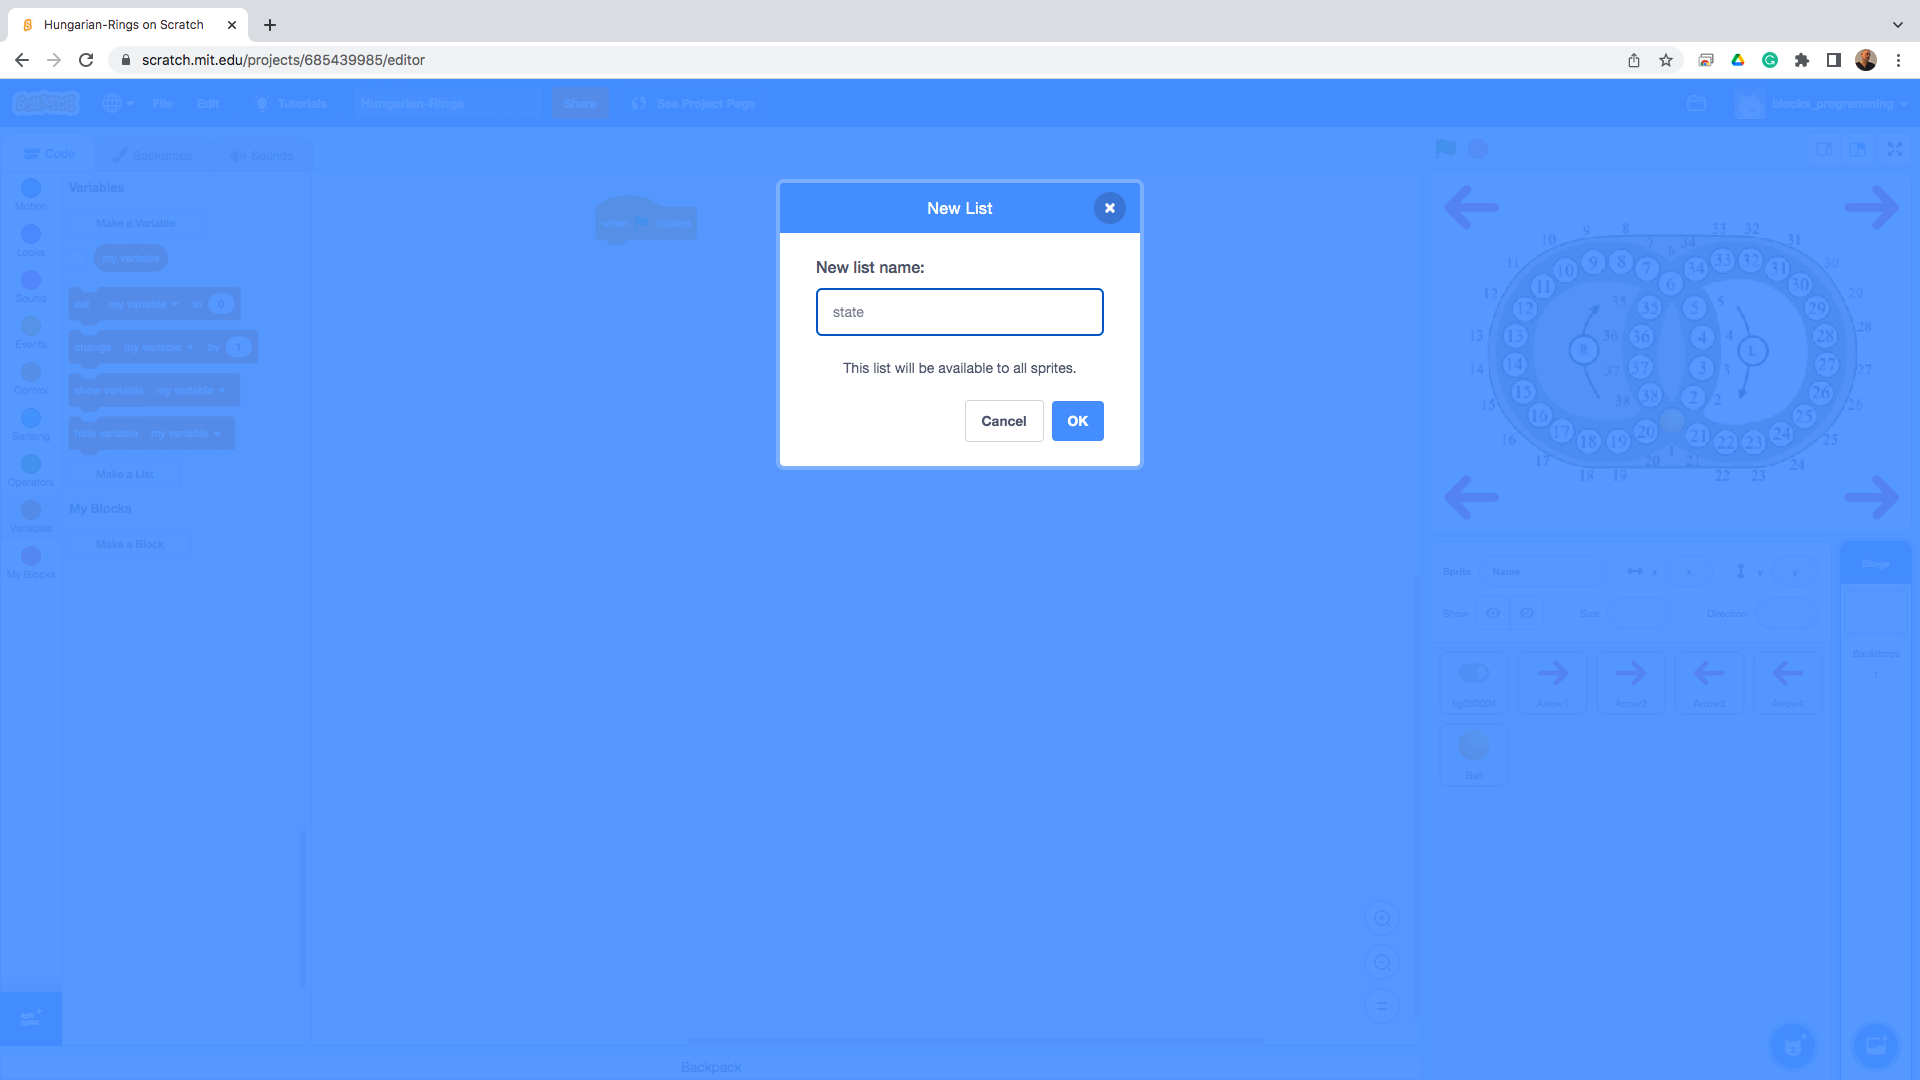
\includegraphics[width=1.0\linewidth,height=0.5\linewidth]{fig050016.png}
  \caption{Списък за състоянието на игралното табло}
\label{fig050016}
\end{figure}

Съдържанието на списъка винаги първо изцяло се изтрива, за да не останат стойности от предишно стартиране. Първите пет позиции са с първия цвят (Фиг. \ref{fig050017}).

\begin{figure}[H]
  \centering
  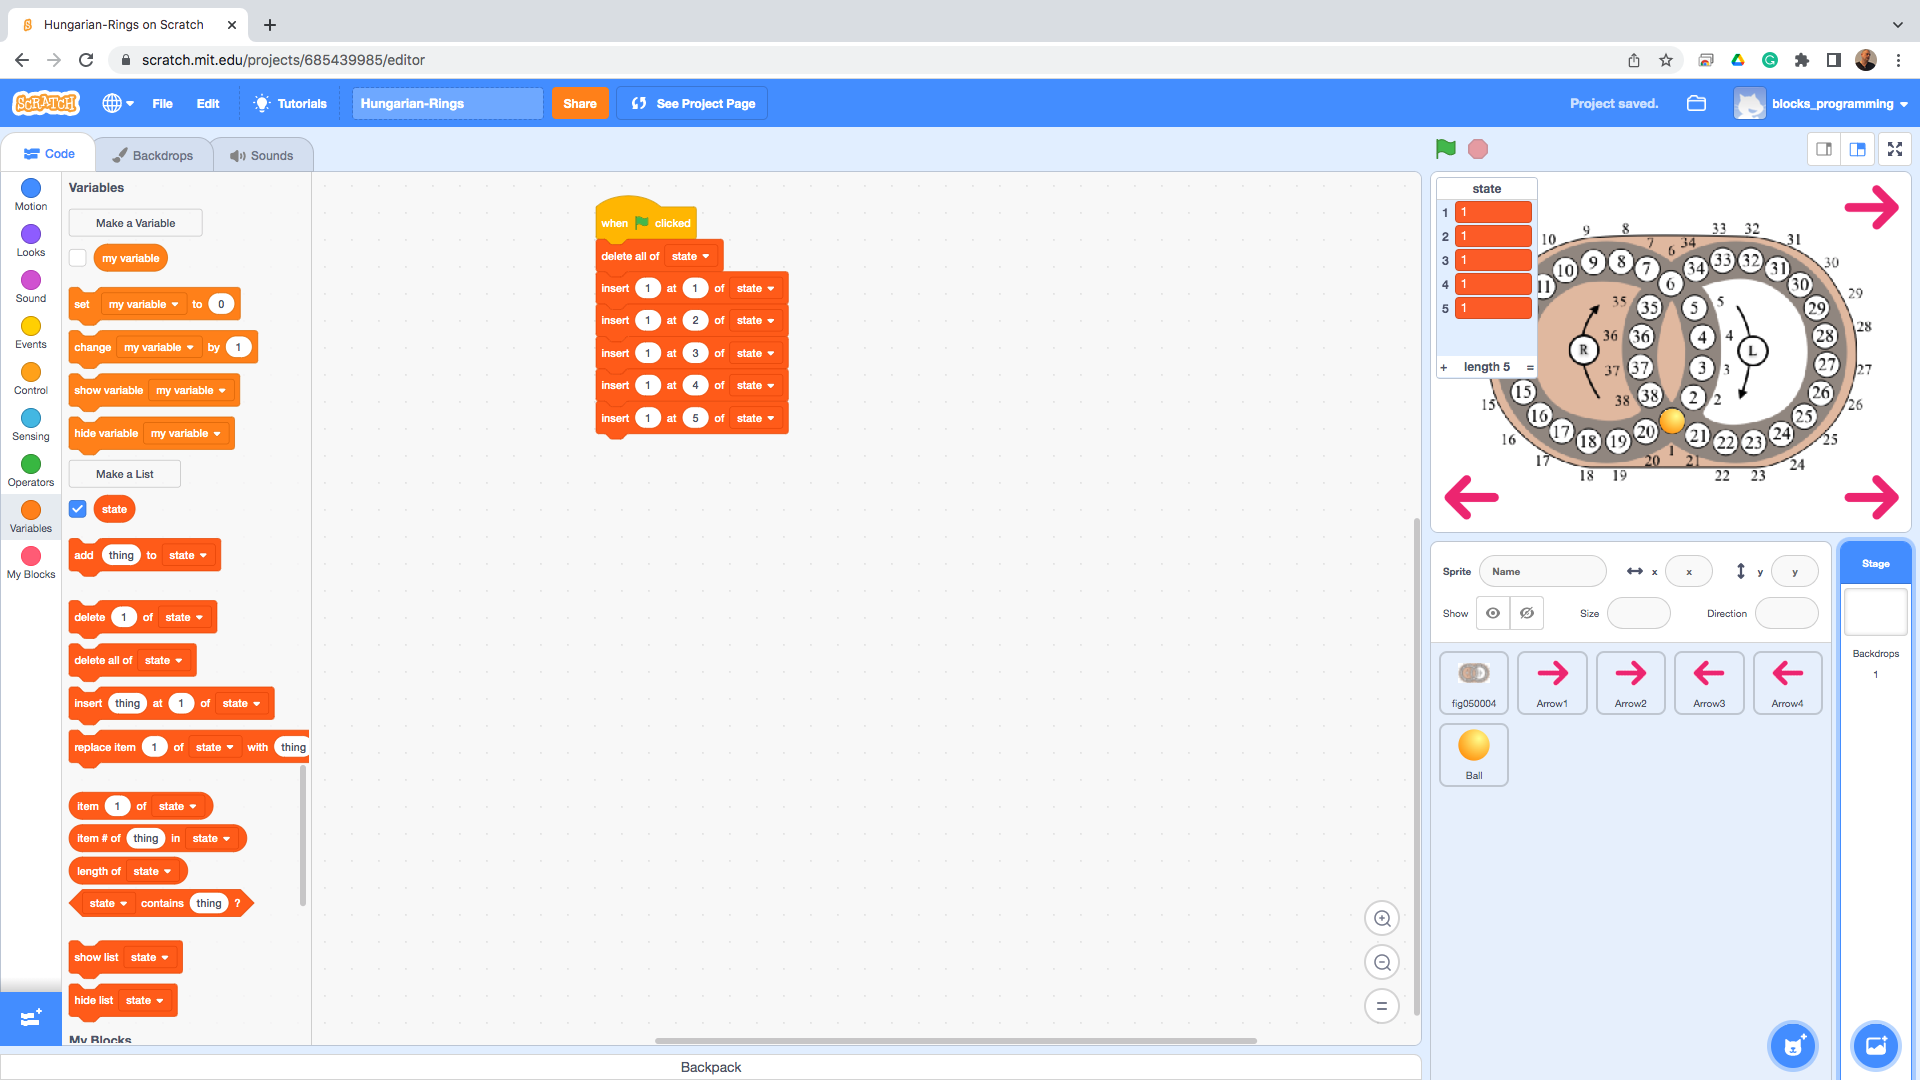
\includegraphics[width=1.0\linewidth,height=0.5\linewidth]{fig050017.png}
  \caption{Цвят на първите пет позиции}
\label{fig050017}
\end{figure}

На шеста позиция се появява четвъртия цвят, след което от седма до шестнадесета позиця е втория цвят. Следват четири позиции от първия цвят, а от двадесет и едно до тридесет са позиции на третия цвят. Всички останали пулове са с четвъртия цвят (Фиг. \ref{fig050018}).

\begin{figure}[H]
  \centering
  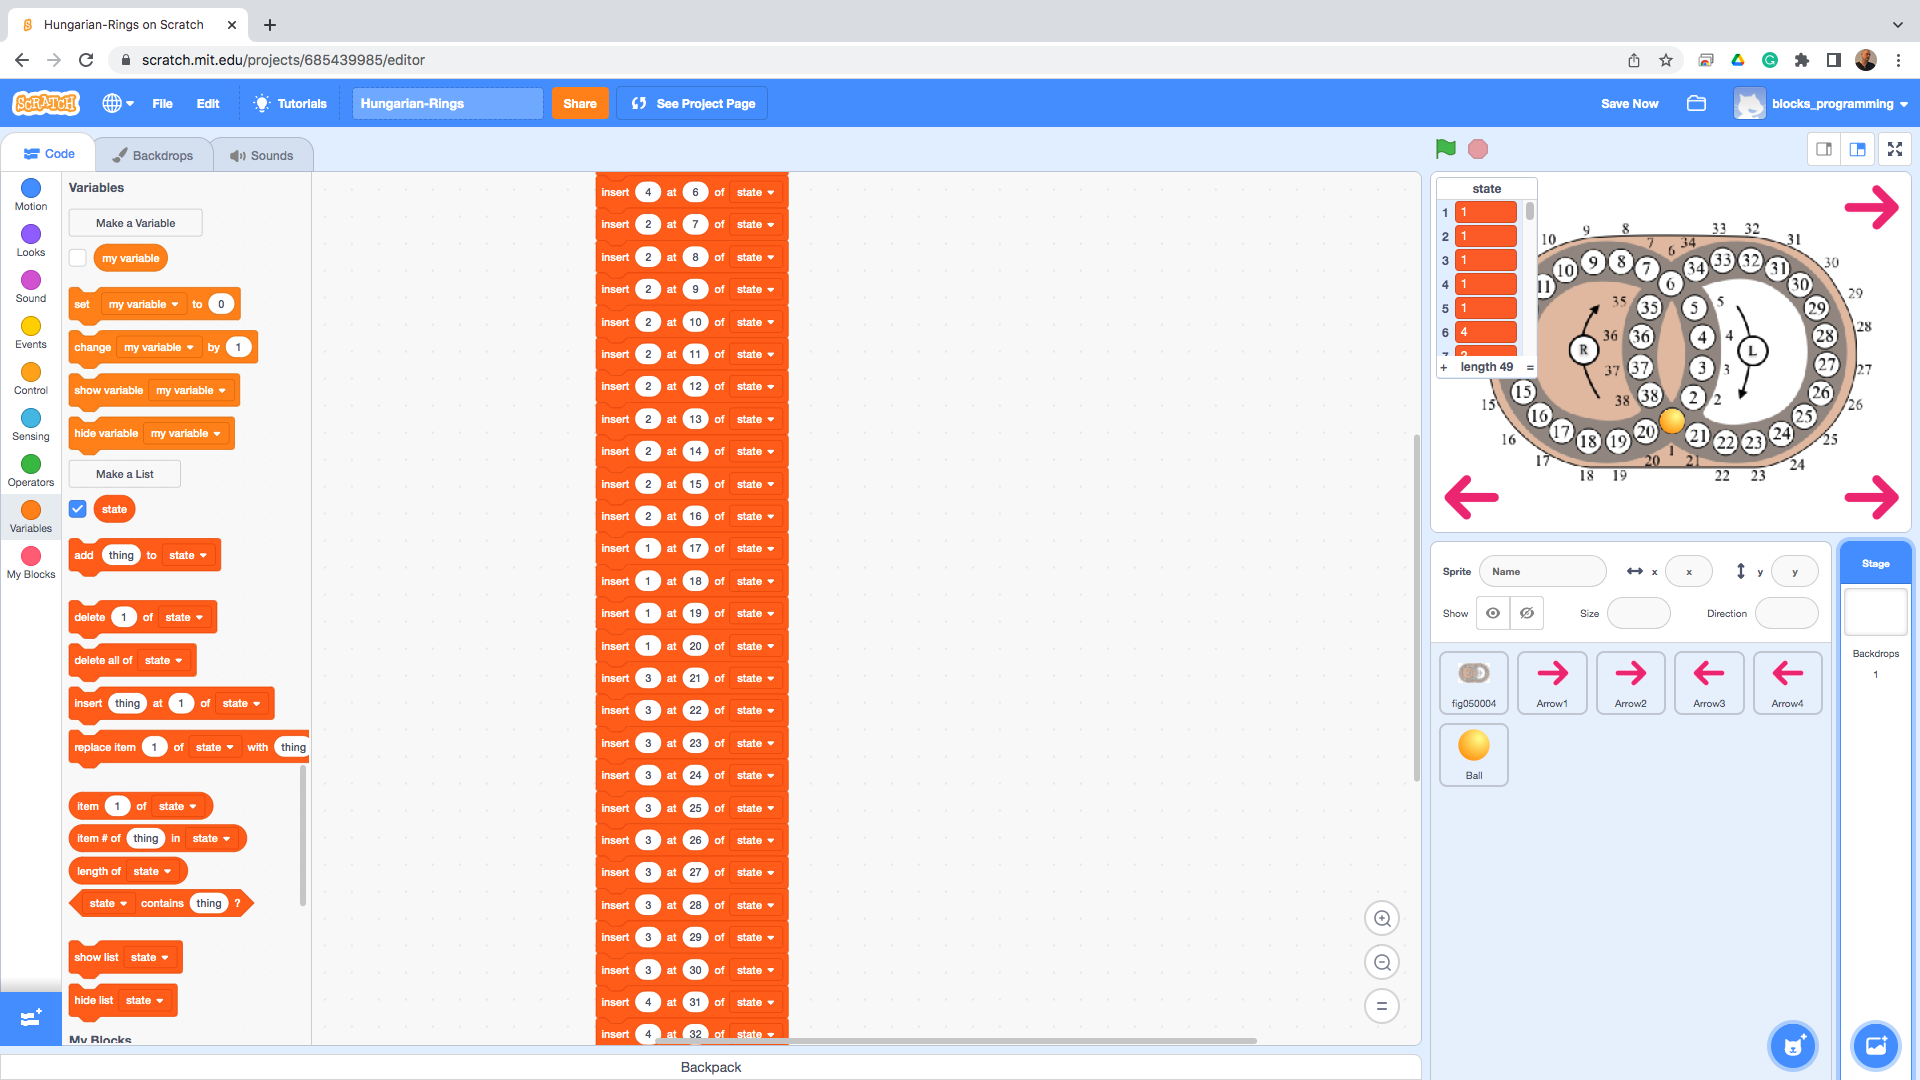
\includegraphics[width=1.0\linewidth,height=0.5\linewidth]{fig050018.png}
  \caption{Общо състояние по цветове}
\label{fig050018}
\end{figure}

След промяна във вътрешното състояние на списъка е важно да се разпрати съобщение за обновяване на всички спрайтове, които визуализират пулчетата (Фиг. \ref{fig050019}). 

\begin{figure}[H]
  \centering
  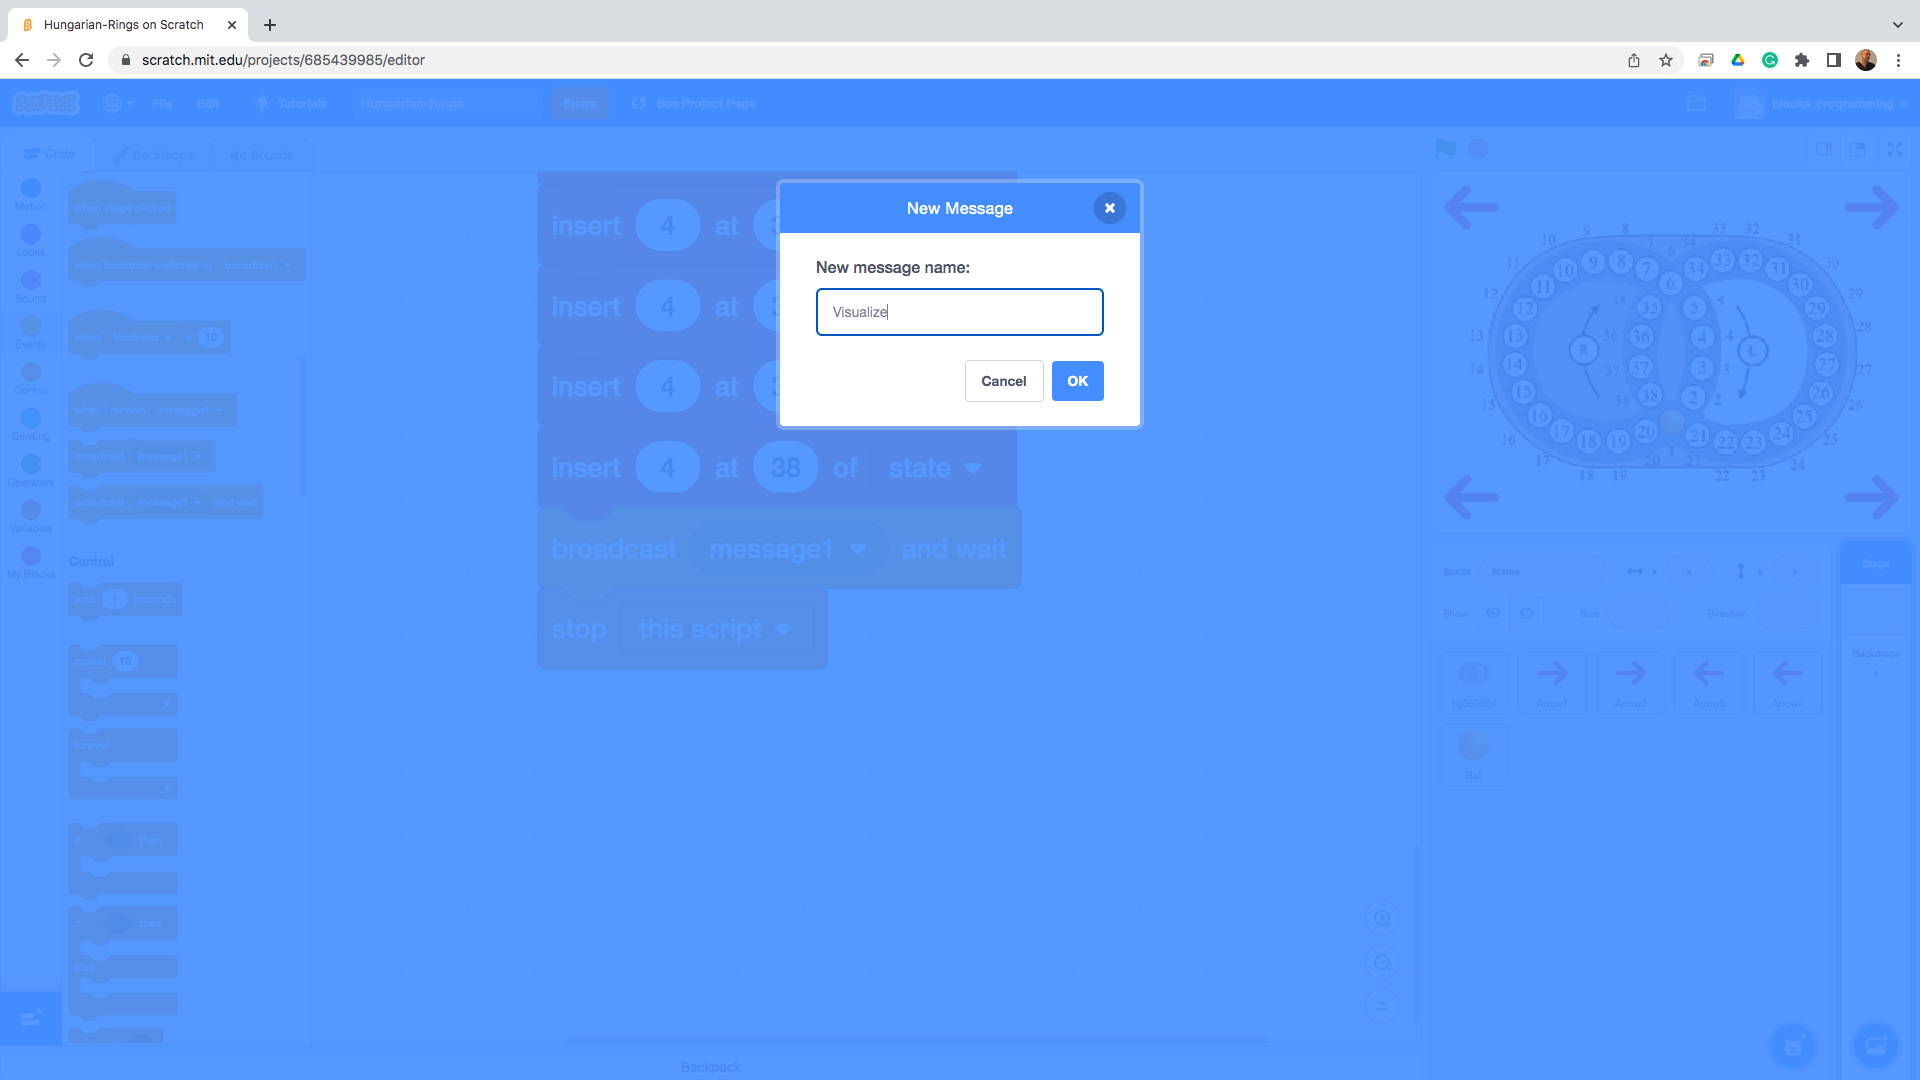
\includegraphics[width=1.0\linewidth,height=0.5\linewidth]{fig050019.png}
  \caption{Съобщение за визуализация}
\label{fig050019}
\end{figure}

Съобщението се изпраща с команда, която изчаква изпълнението му (Фиг. \ref{fig050020}). Всяко от 38-те пулчета ще се абонира за получаване на това съобщение. 

\begin{figure}[H]
  \centering
  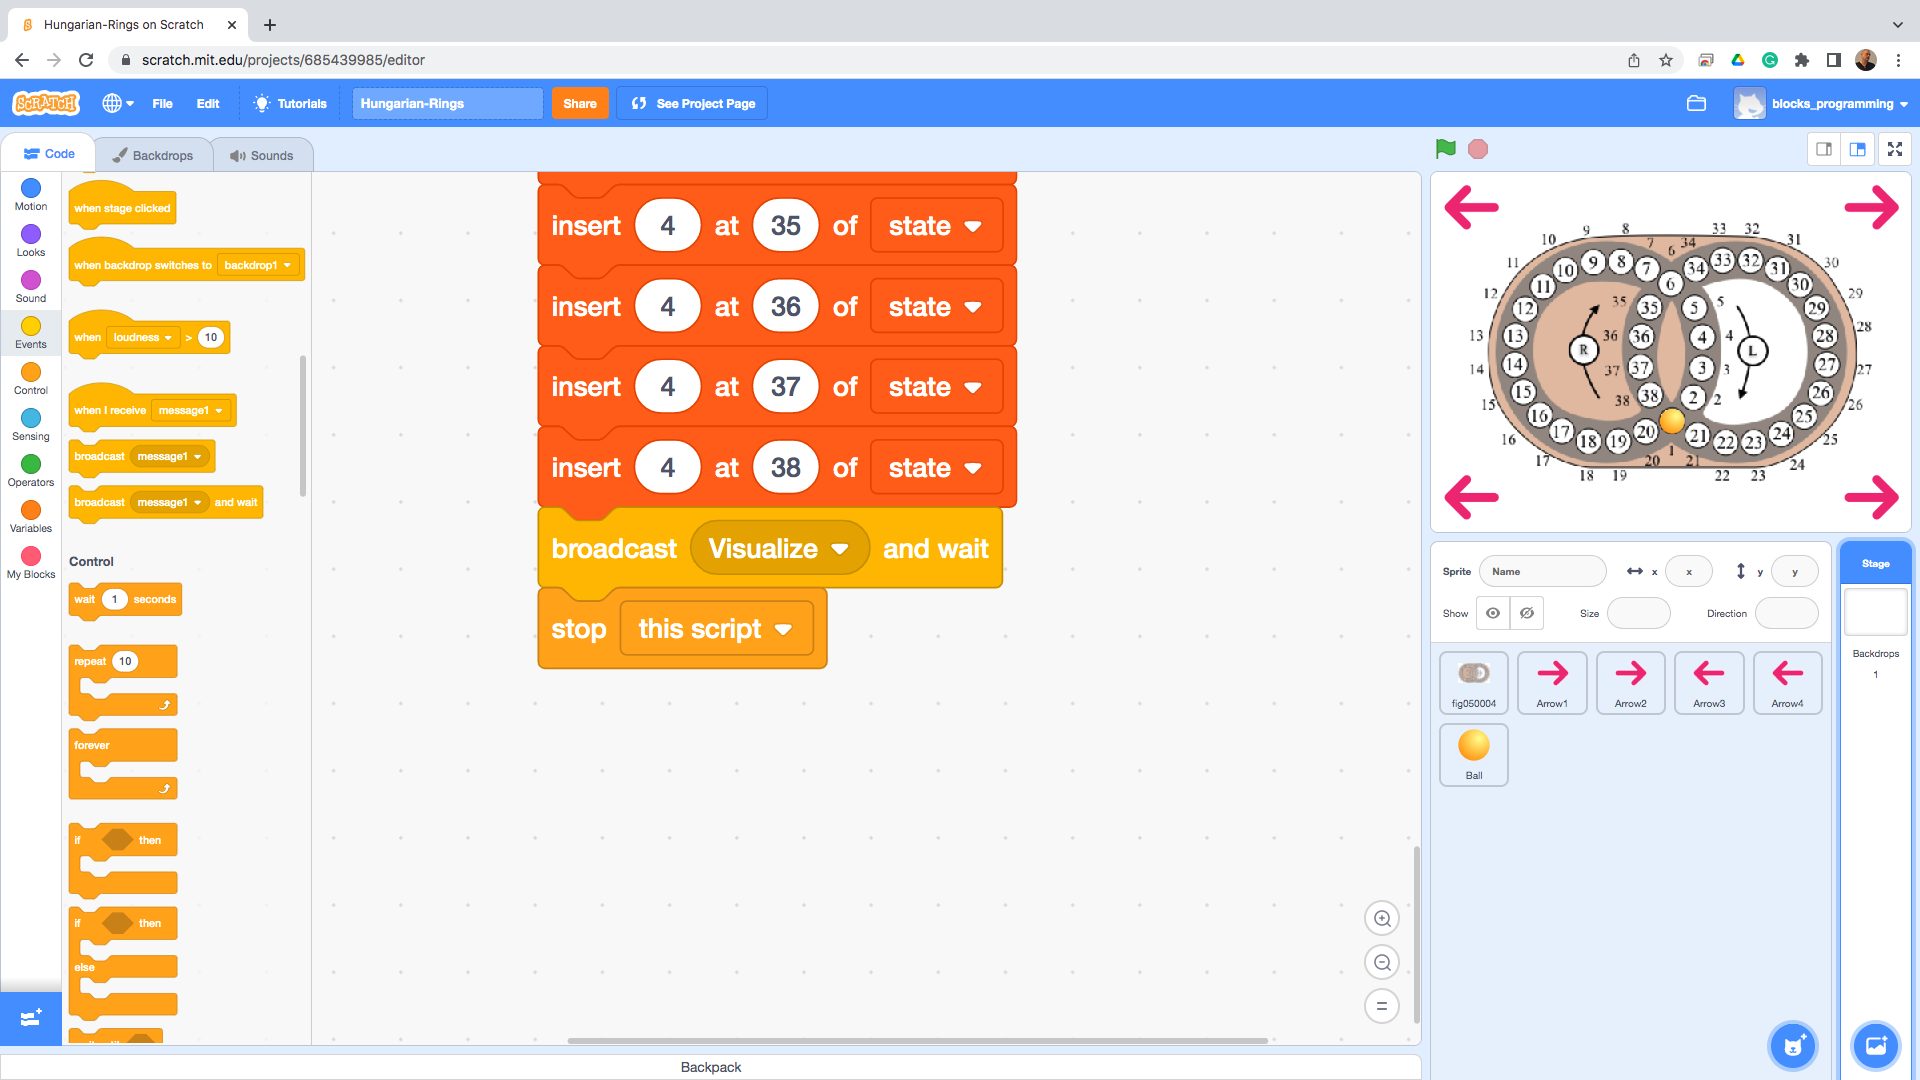
\includegraphics[width=1.0\linewidth,height=0.5\linewidth]{fig050020.png}
  \caption{Изпращане с изчакване}
\label{fig050020}
\end{figure}

Преди да започне копирането на първия пул, така че да се размножи още 37 пъти, следва да се състави кодът, който ще прослушва за съобщение за изрисуване. Първо се написва този код, така че той да се размножи 37 пъти при дублирането на спрайта. Пул с номер едно прави четири проверки в елемент от списъка с номер едно. Според числото в списъка се избира един от четирите възможни цвята (Фиг. \ref{fig050021}).

\begin{figure}[H]
  \centering
  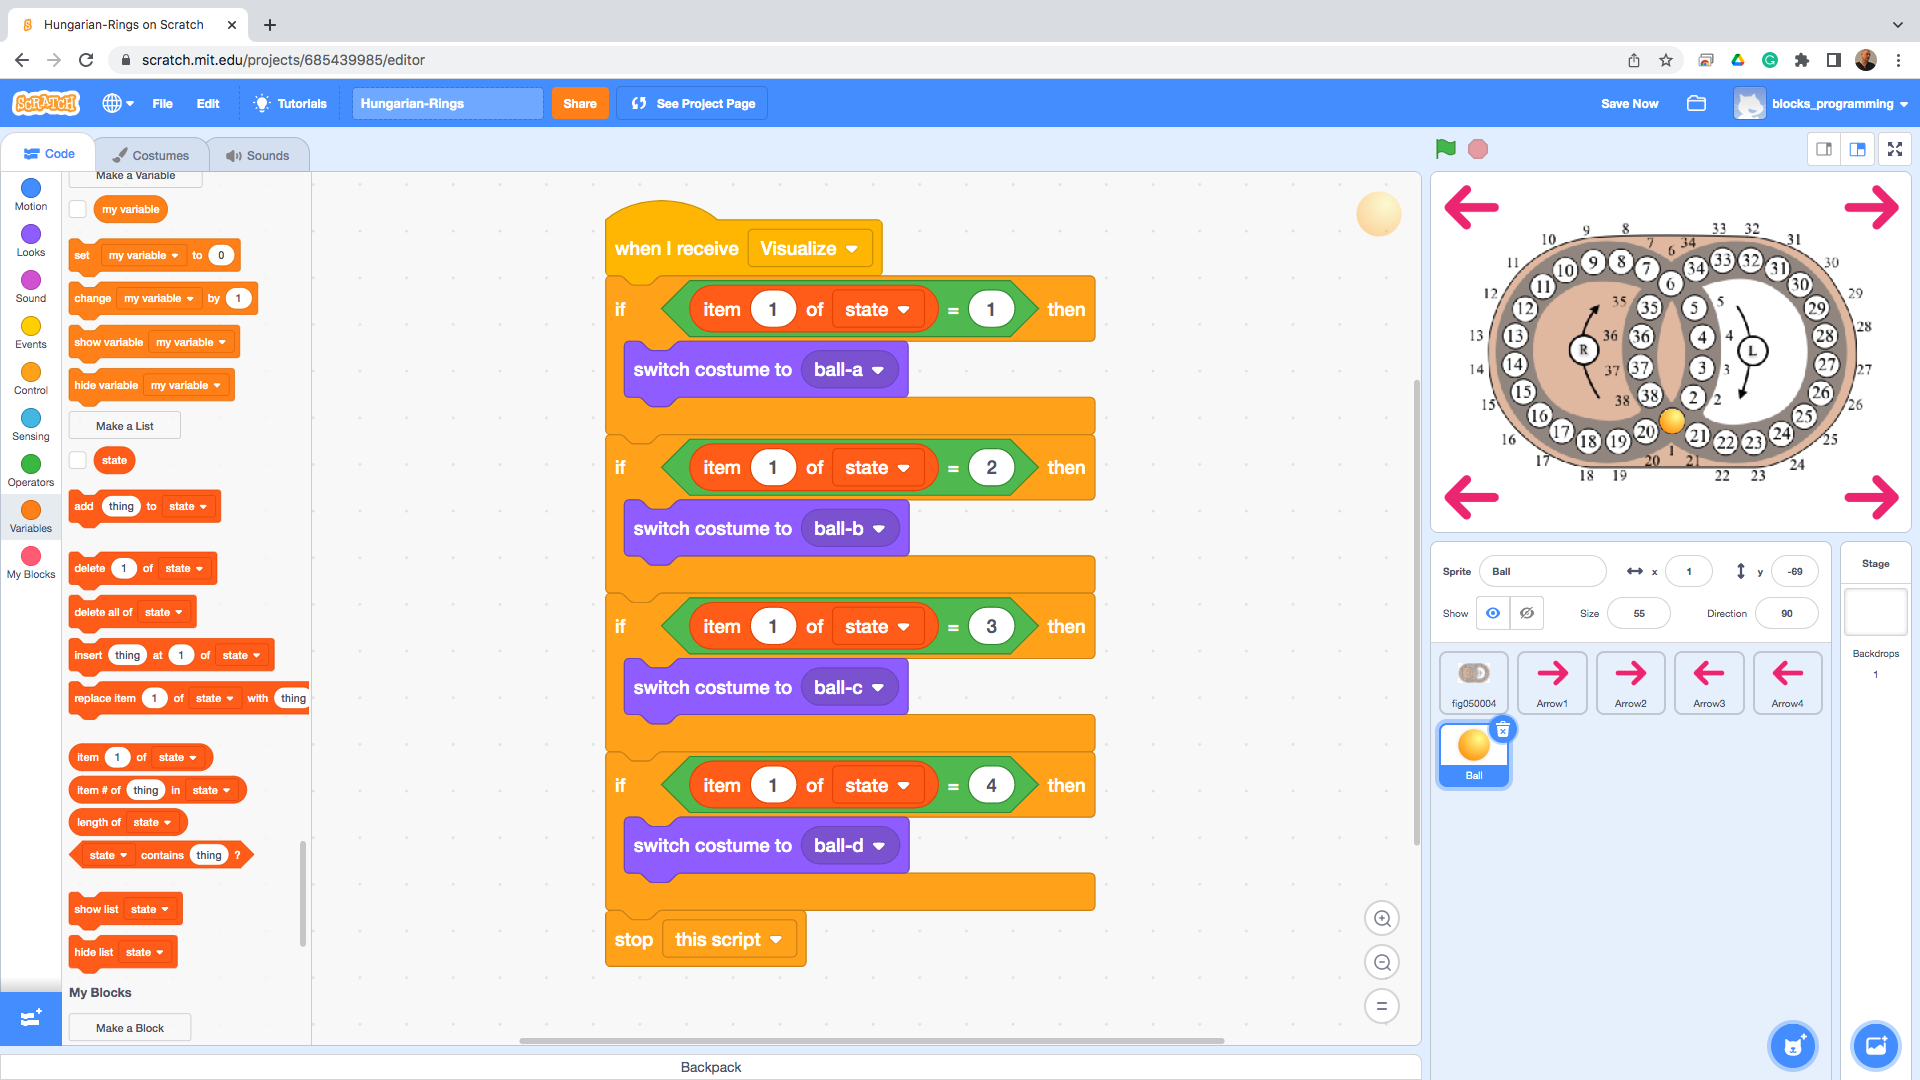
\includegraphics[width=1.0\linewidth,height=0.5\linewidth]{fig050021.png}
  \caption{Инструкции за прерисуване на пула}
\label{fig050021}
\end{figure}

Така подготвеният първи пул може да се дублира и разпространи по цялата схема, като се съобразяват цветовете на отделните позиции (Фиг. \ref{fig050022}). 

\begin{figure}[H]
  \centering
  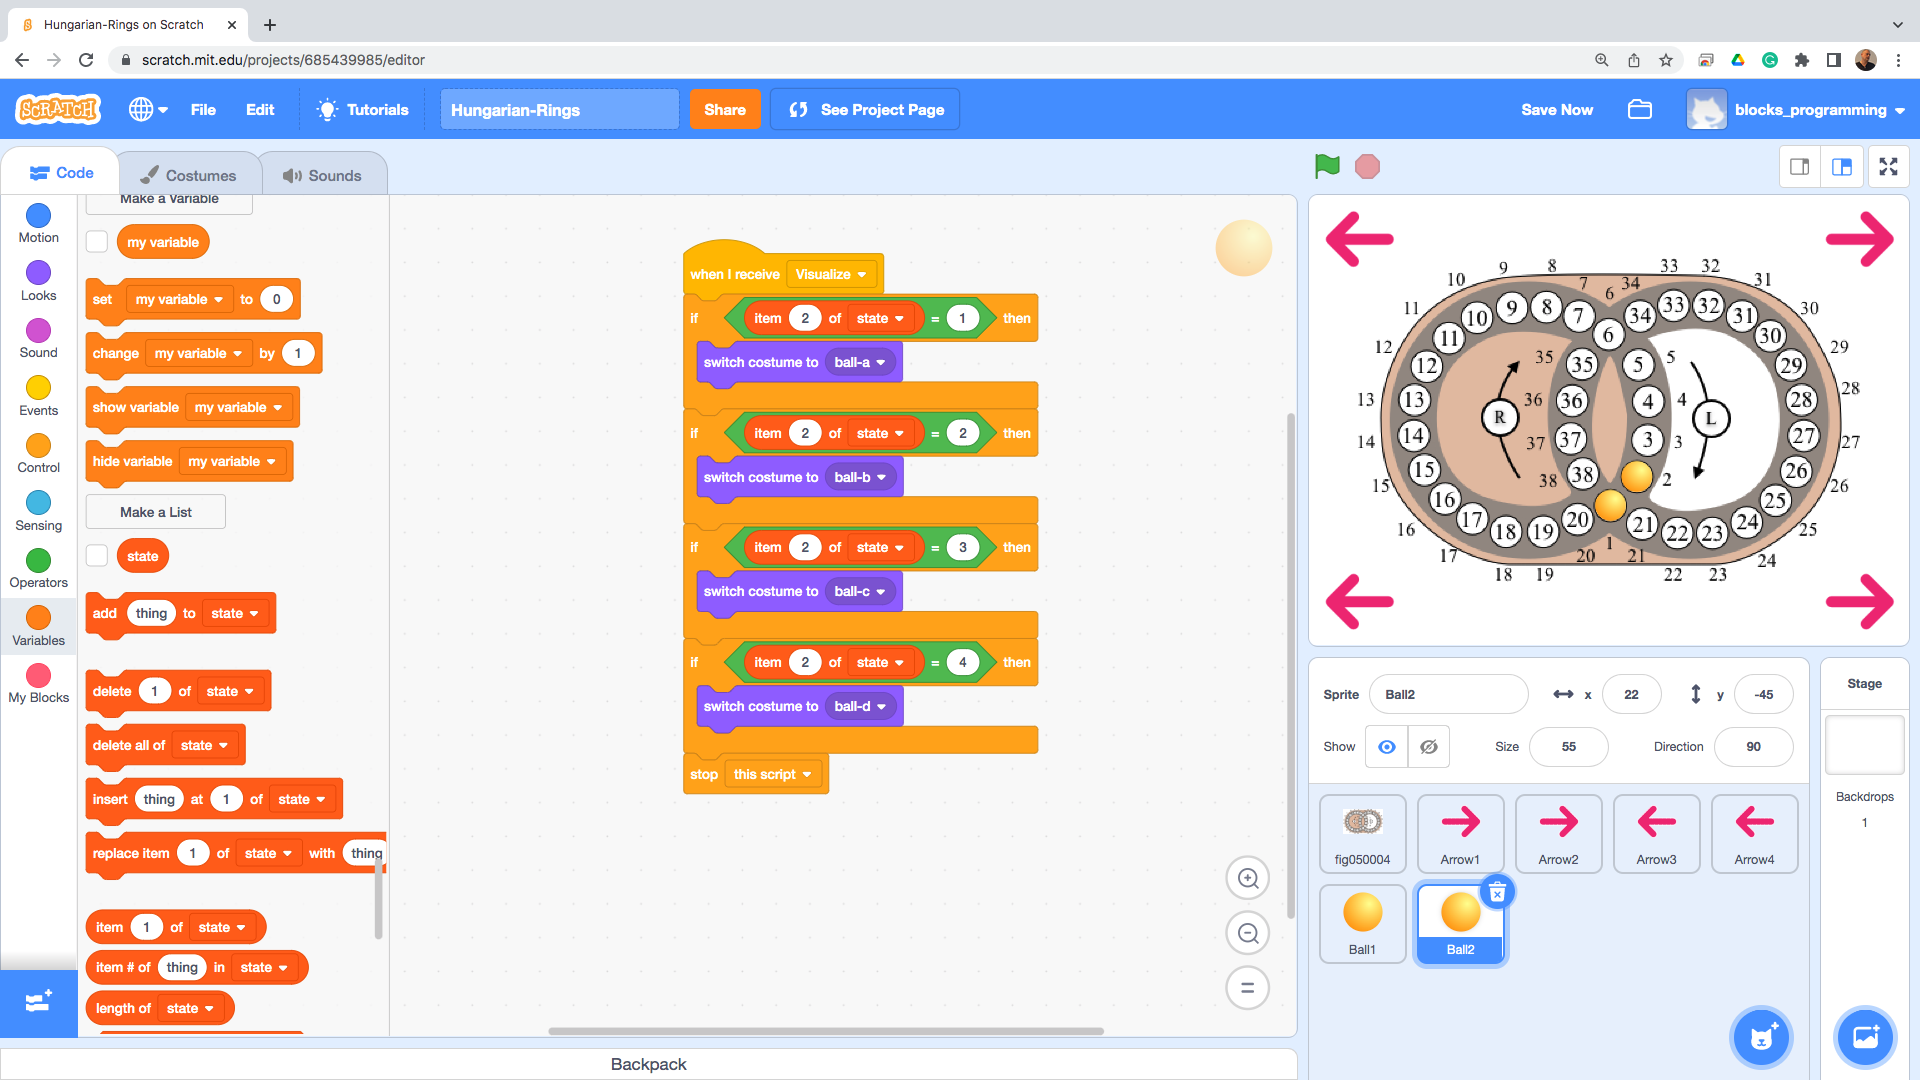
\includegraphics[width=1.0\linewidth,height=0.5\linewidth]{fig050022.png}
  \caption{Дублиране на пула}
\label{fig050022}
\end{figure}

При подреждането на всичките 38 пула, върху схемата на играта, ясно се оформят двата ринга (Фиг. \ref{fig050023}).

\begin{figure}[H]
  \centering
  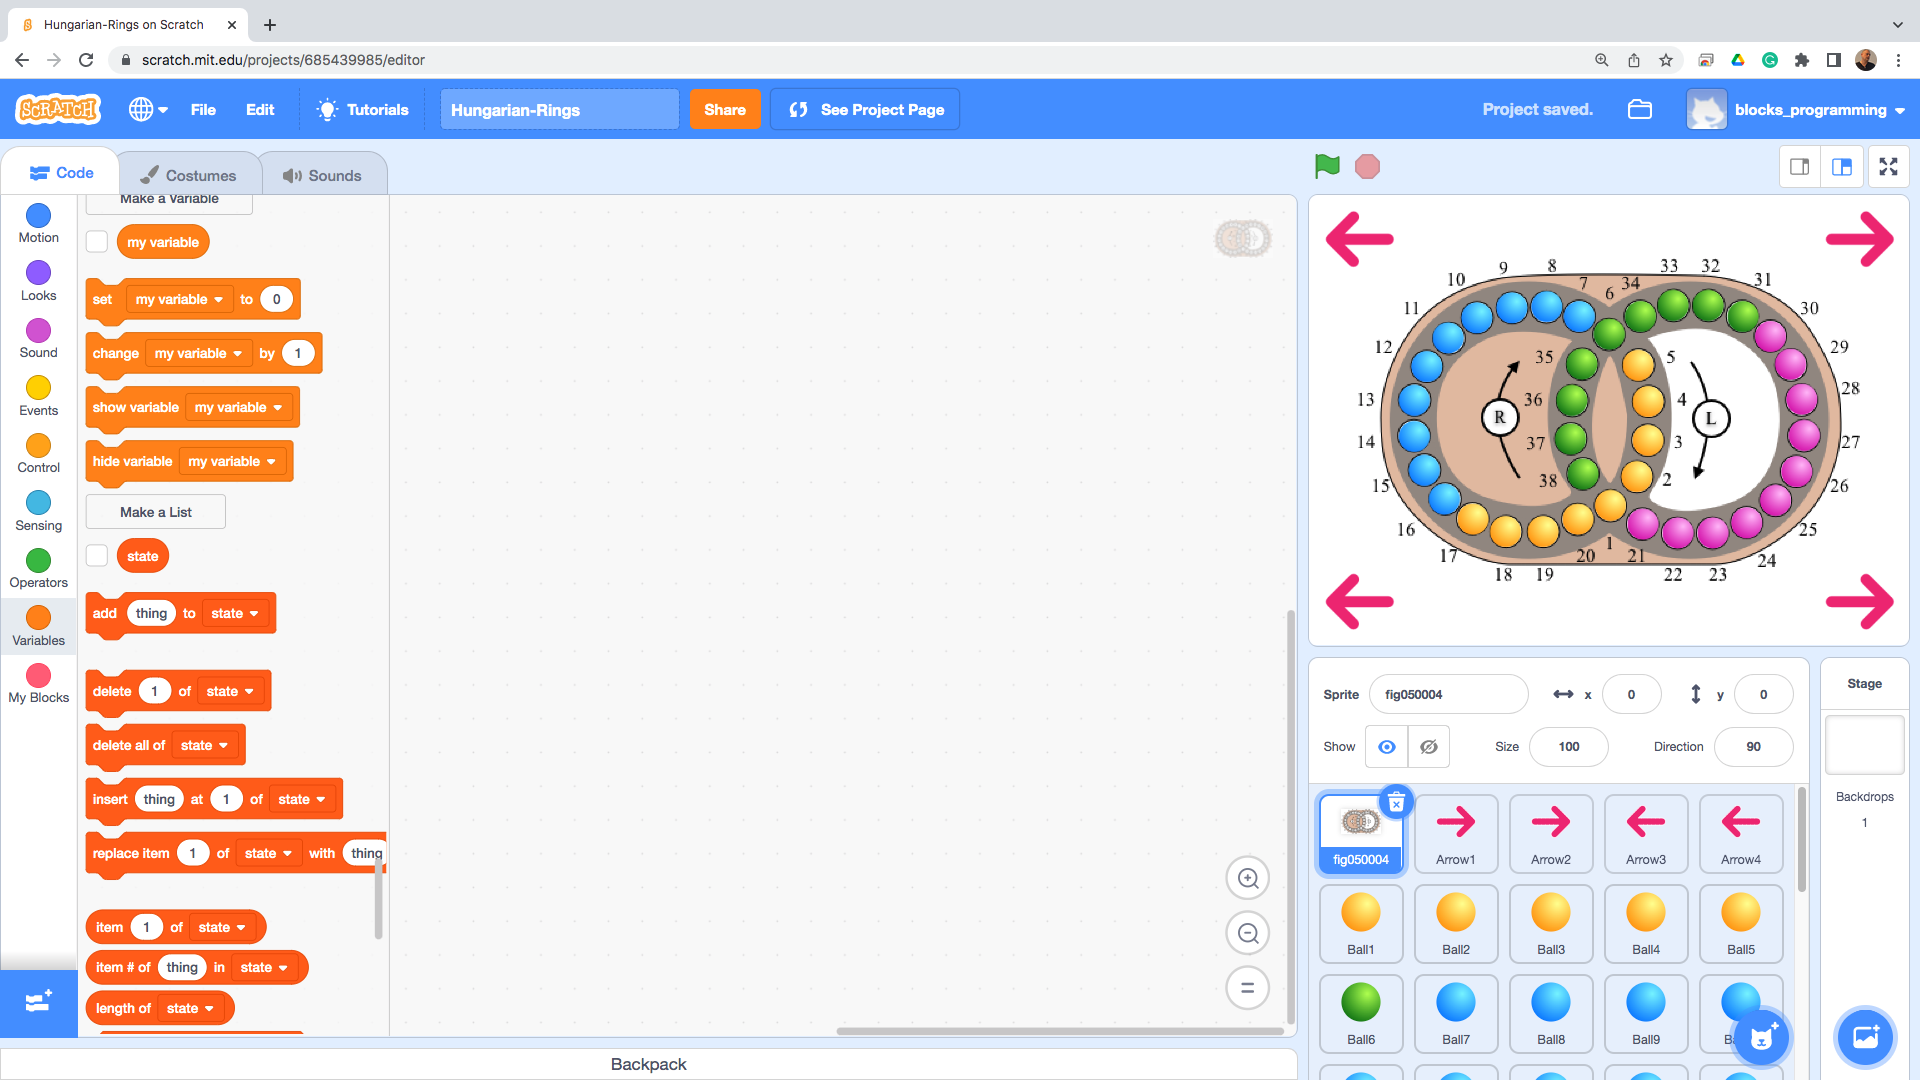
\includegraphics[width=1.0\linewidth,height=0.5\linewidth]{fig050023.png}
  \caption{Дублиране на пула}
\label{fig050023}
\end{figure}

Схемата на играта, на този етап, е само помощна (Фиг. \ref{fig050024}), когато се премахне номерацията, същото изображение може да се ползва за фон на двата ринга от пулове.

\begin{figure}[H]
  \centering
  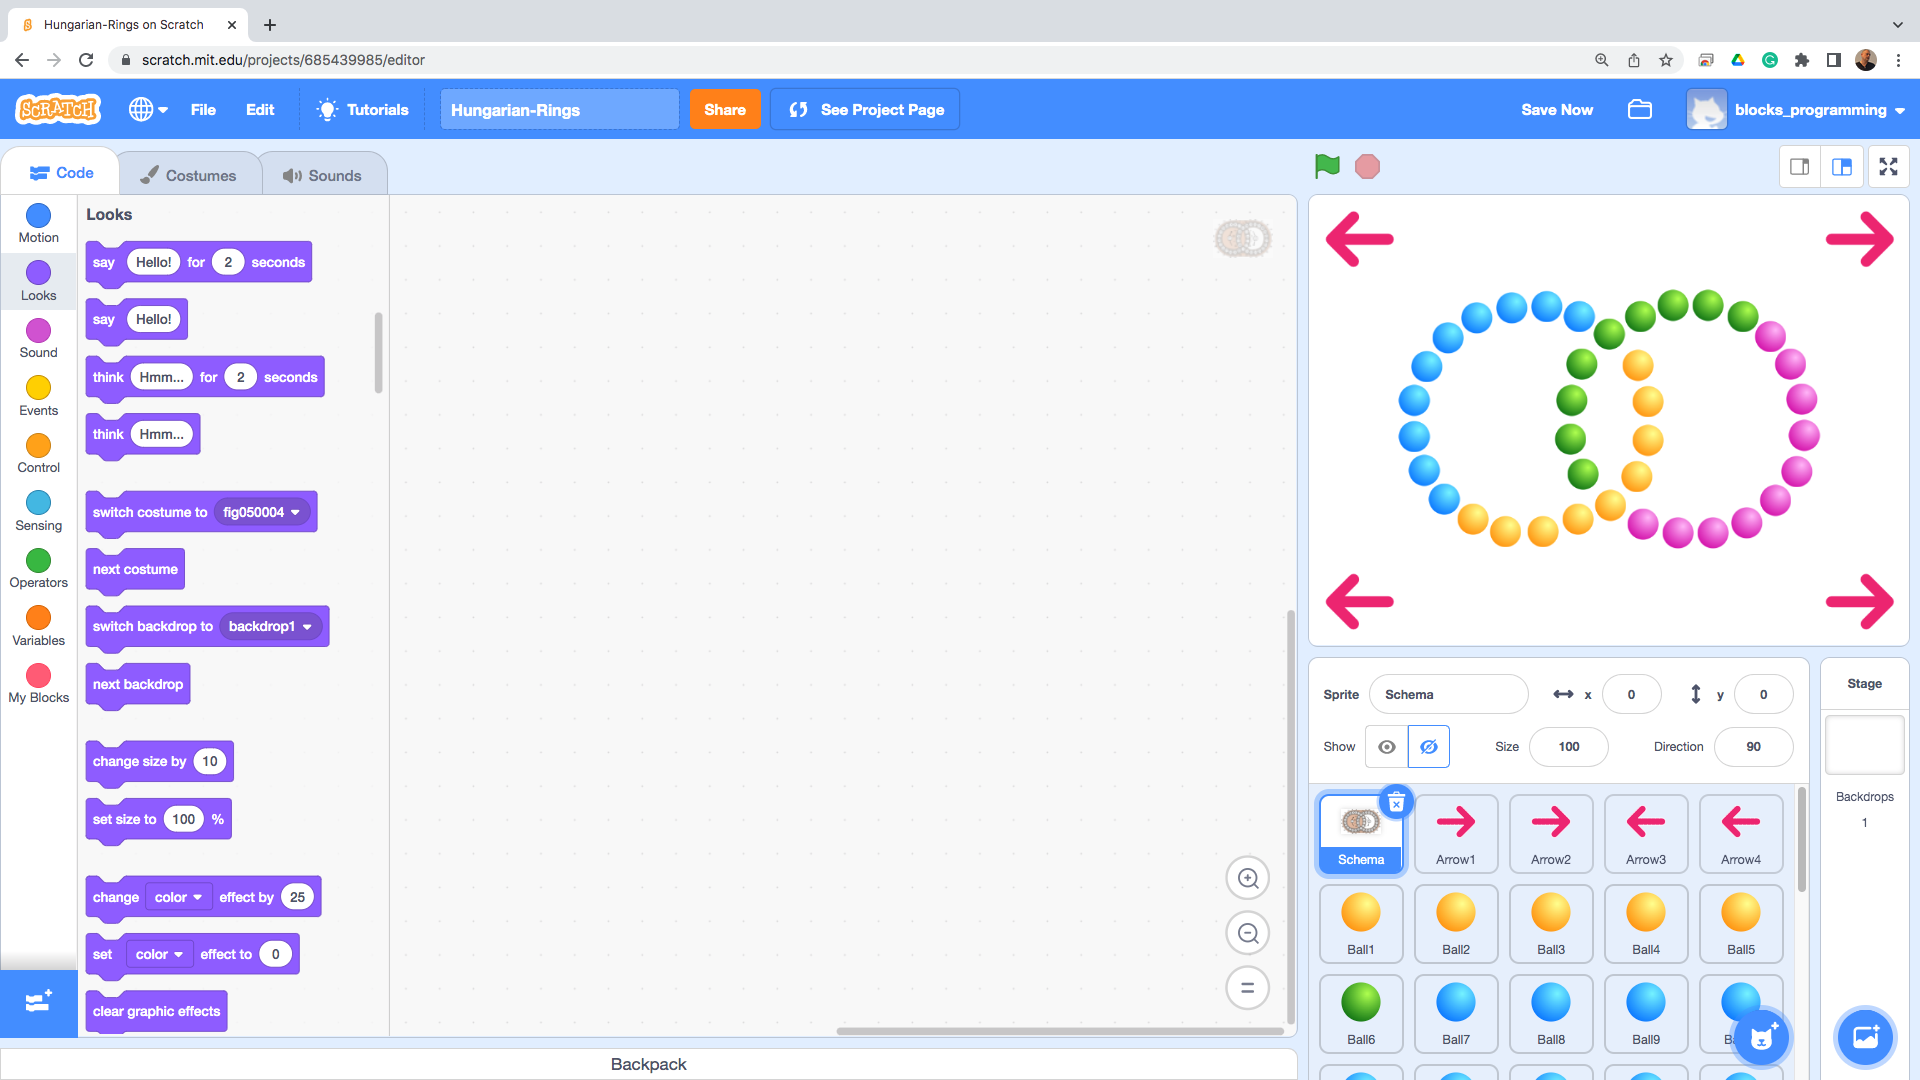
\includegraphics[width=1.0\linewidth,height=0.5\linewidth]{fig050024.png}
  \caption{Премахване на схемата}
\label{fig050024}
\end{figure}

\section{Алгоритми за манипулация на игралното поле}

При натискане на първата стрелка (горе-дясно) първо се разпространява съобщение за извършване на ротация в десния ринг, по часовниковата стрелка (Фиг. \ref{fig050025}). След това се разпространява съобщение за обновяване на цялото визуално пространство.

\begin{figure}[H]
  \centering
  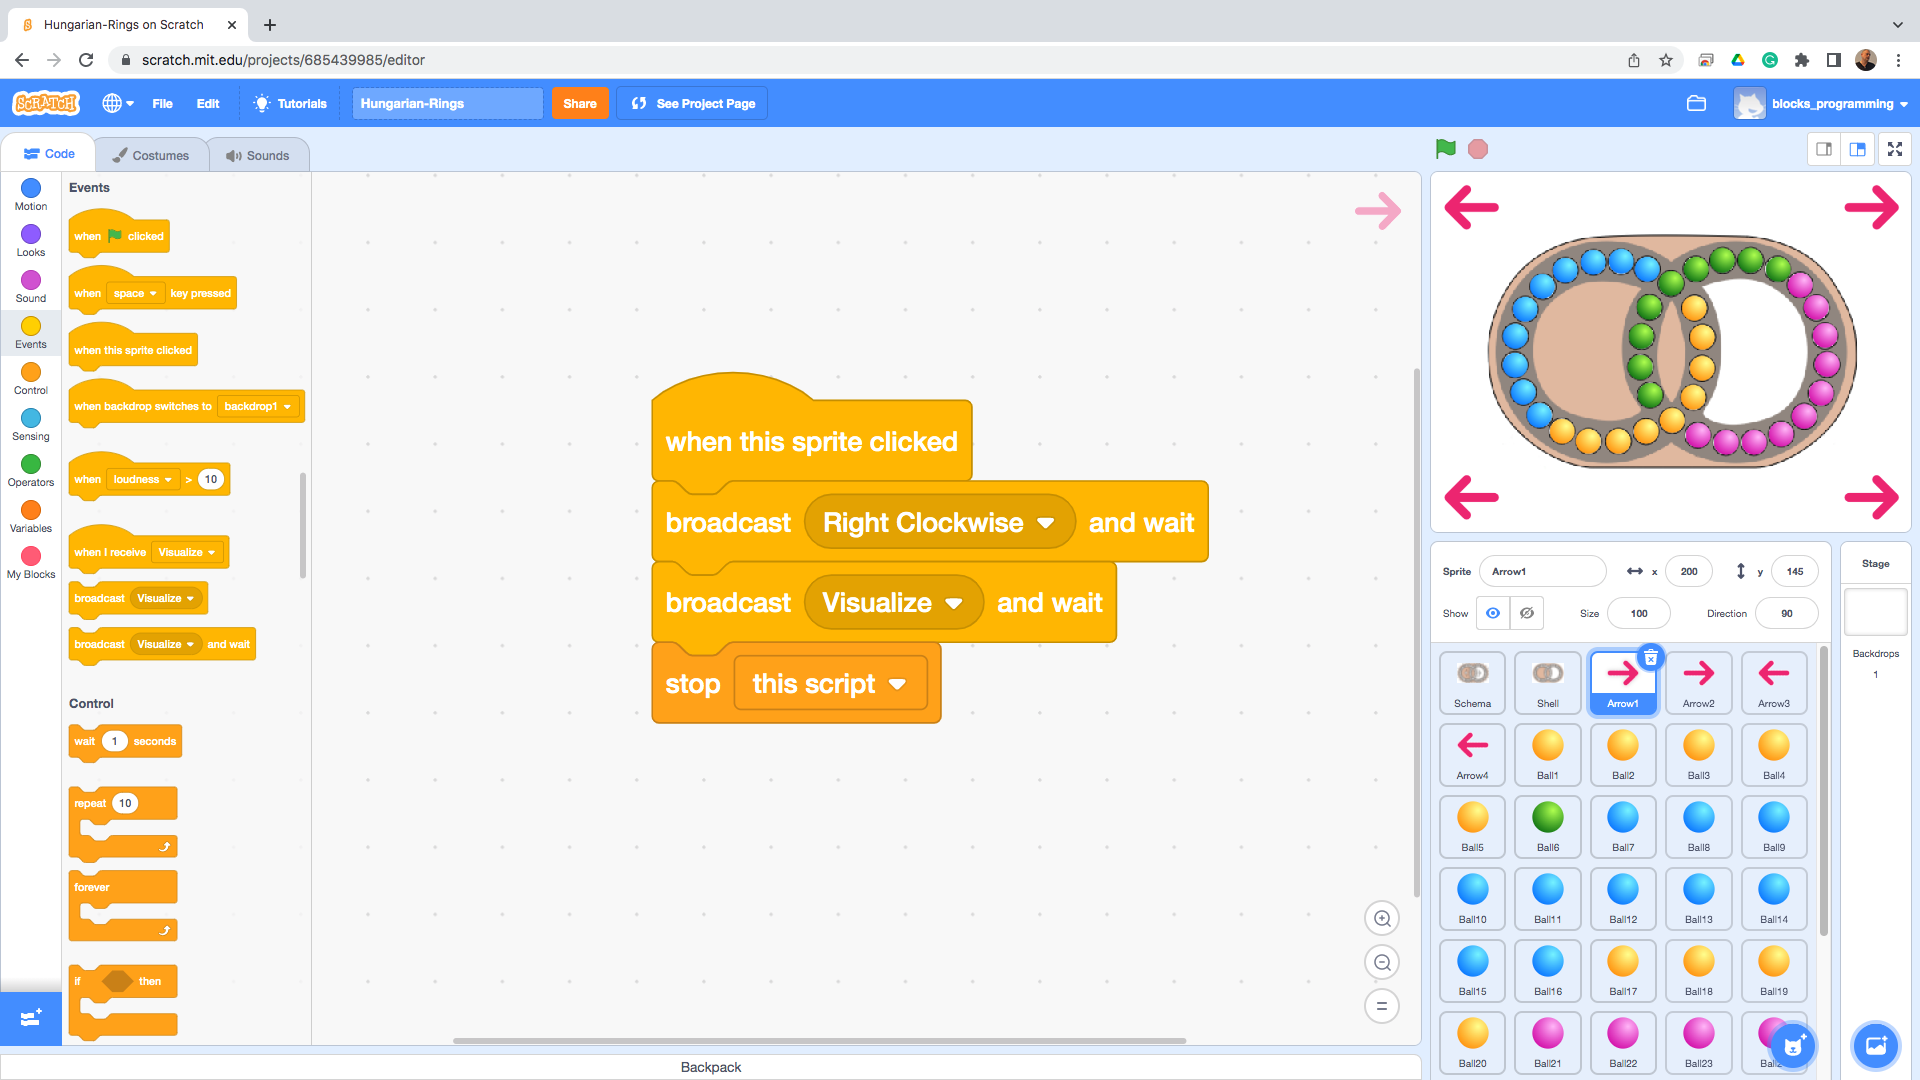
\includegraphics[width=1.0\linewidth,height=0.5\linewidth]{fig050025.png}
  \caption{Съобщение за ротация и изчертаване}
\label{fig050025}
\end{figure}

По абсолютно аналогичен начин се подават съобщения и от другите три стрелки, като съобщенията указват ринга и посоката на въртене. След първоначалната инициализация на списъкът с цветовете, следва визуализация, след това се дава малък интервал, така че потребителят да види началното състояние и се изпраща съобщение за разбъркване на пъзела (Фиг. \ref{fig050026}).

\begin{figure}[H]
  \centering
  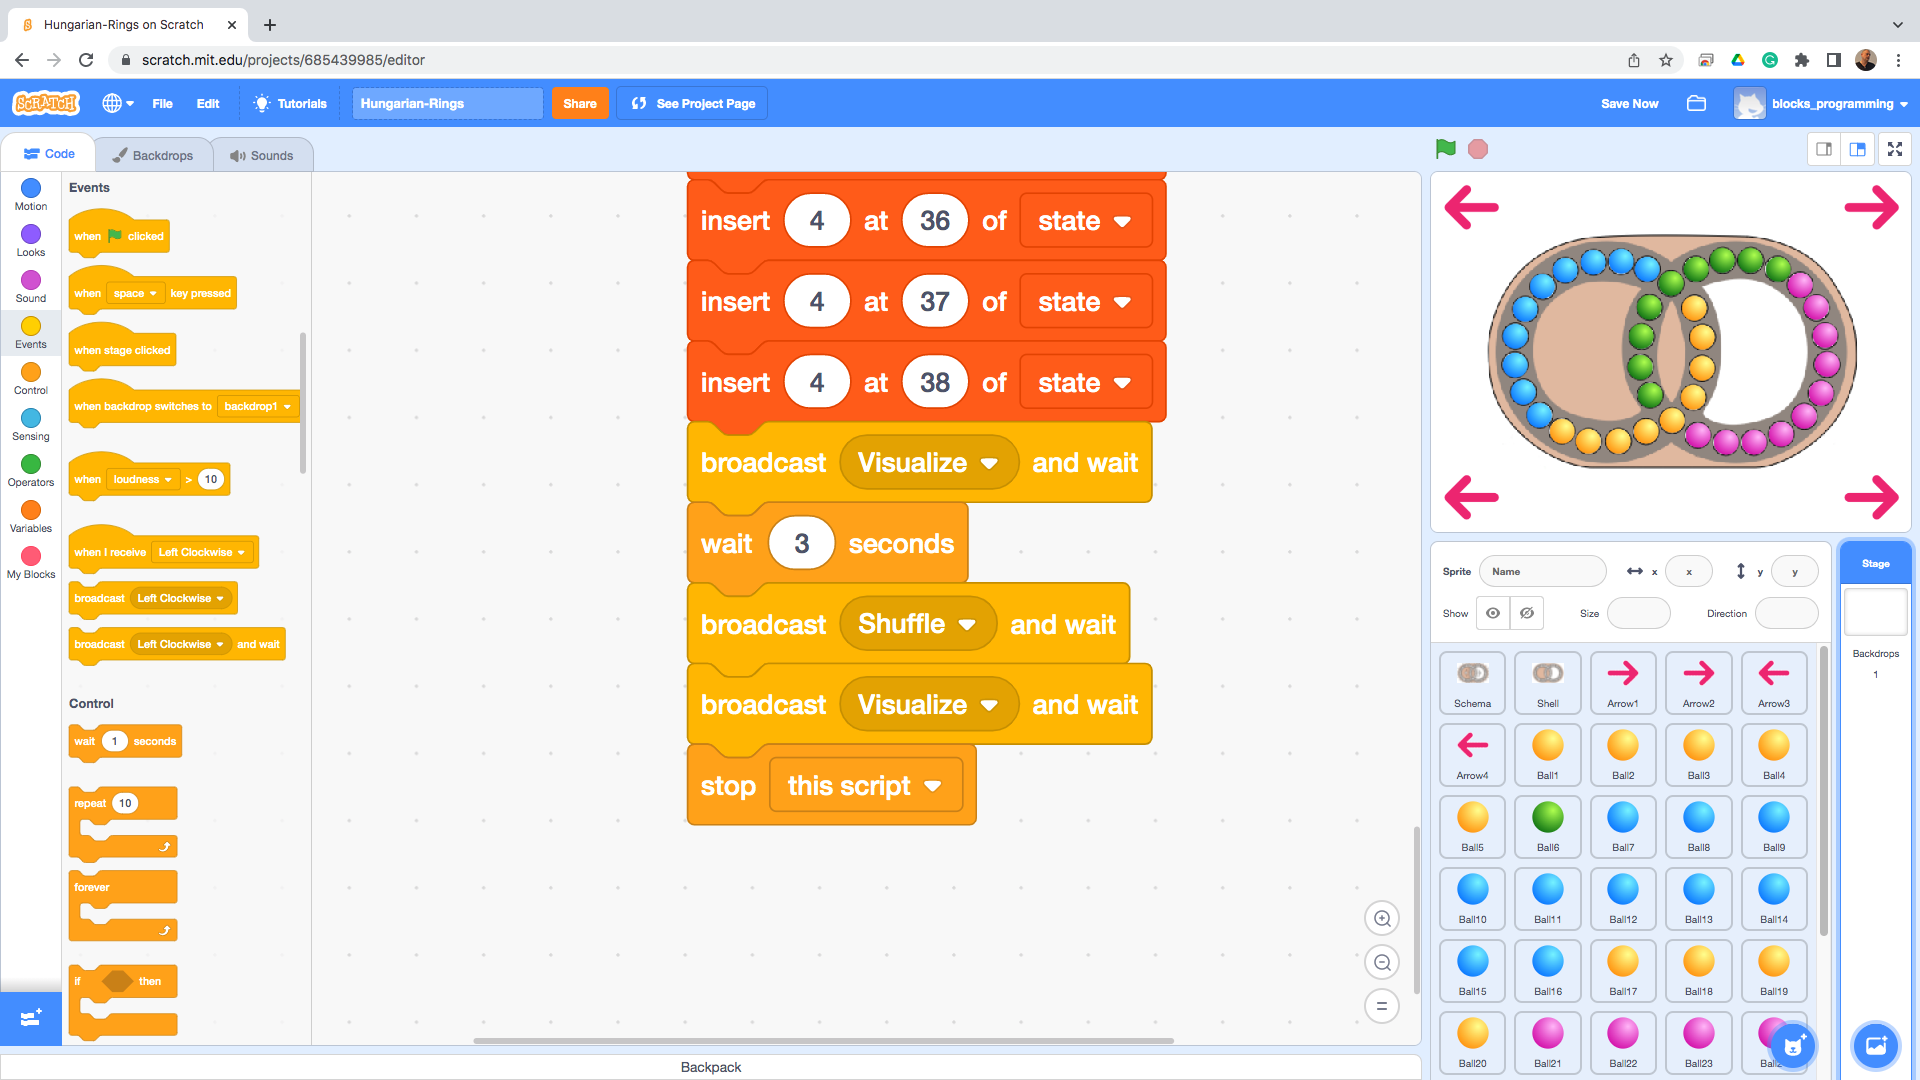
\includegraphics[width=1.0\linewidth,height=0.5\linewidth]{fig050026.png}
  \caption{Изпращане на съобщение за разбъркване}
\label{fig050026}
\end{figure}

Разбъркването на пъзела може да се случи по много начини, но най-удачният е чрез случайно извикване на четирите възможности за ротация. Този алгоритъм също ще бъде сглобен в пространството на основната сцена, а не като код за някои от спрайтовете. Алгоритъмът започва при получаване на съобщението за разбъркване. Тъй като пулчетата са 38 на брой, средно статистически може да се даде шанс на всяко да се мръдне 10 пъти. Това подсказва, че общият брой случайни движения може да се определи на 380, което е 38 по 10 (Фиг. \ref{fig050027}).

\begin{figure}[H]
  \centering
  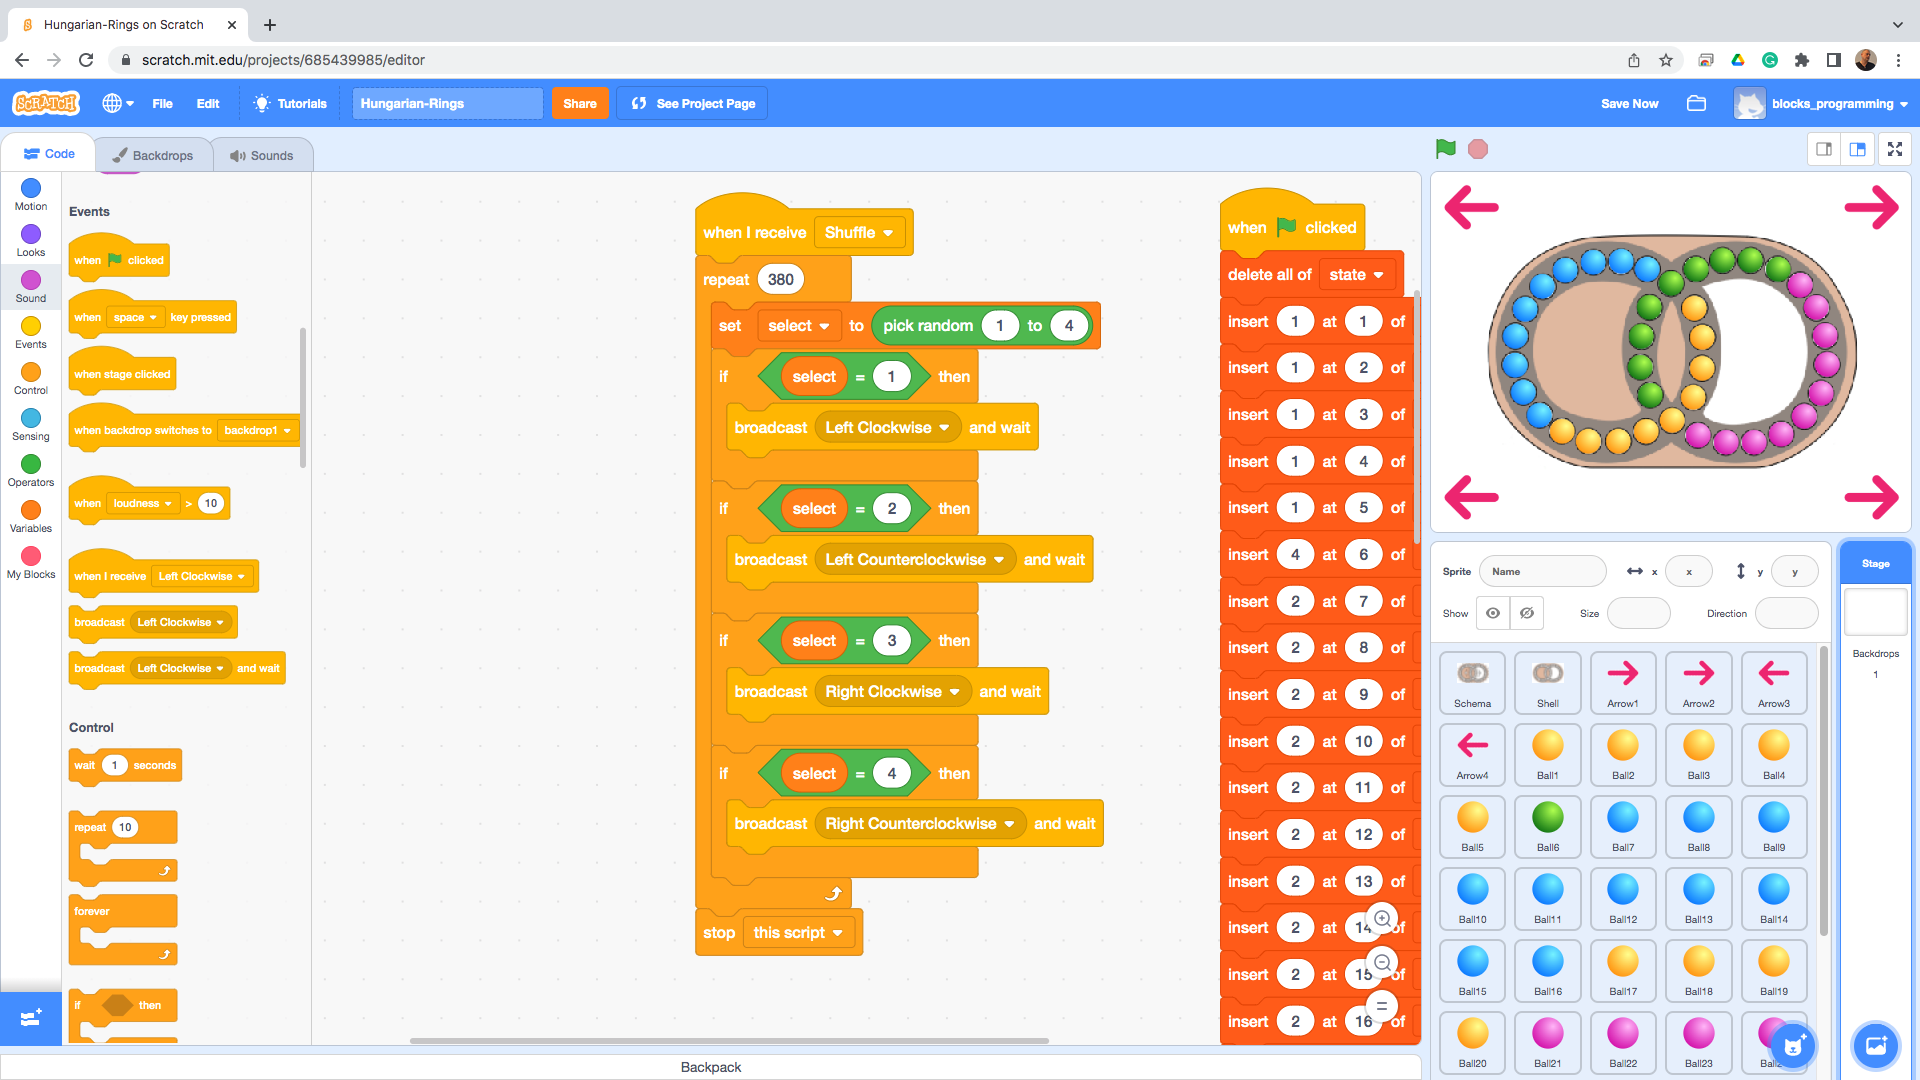
\includegraphics[width=1.0\linewidth,height=0.5\linewidth]{fig050027.png}
  \caption{Алгоритъм за разбъркване}
\label{fig050027}
\end{figure}

Инструкциите за ротация на ринговете също ще бъдат поместени в пространството на сцената. Всяка от четирите стрелки изпраща подходящо съобщение. Прихванатото съобщение за ротация трябва да промени съдържанието на списъка по такъв начин, че то да отразява желаната ротация. За правилно извършване на разместванията, схемата на играта е от голяма полза, защото указва кой номер къде трябва да отиде. 

Ротацията на левия ринг, по часовниковата стрелка се извършва със следната последователност от действия (Фиг. \ref{fig050028}).

\begin{figure}[H]
  \centering
  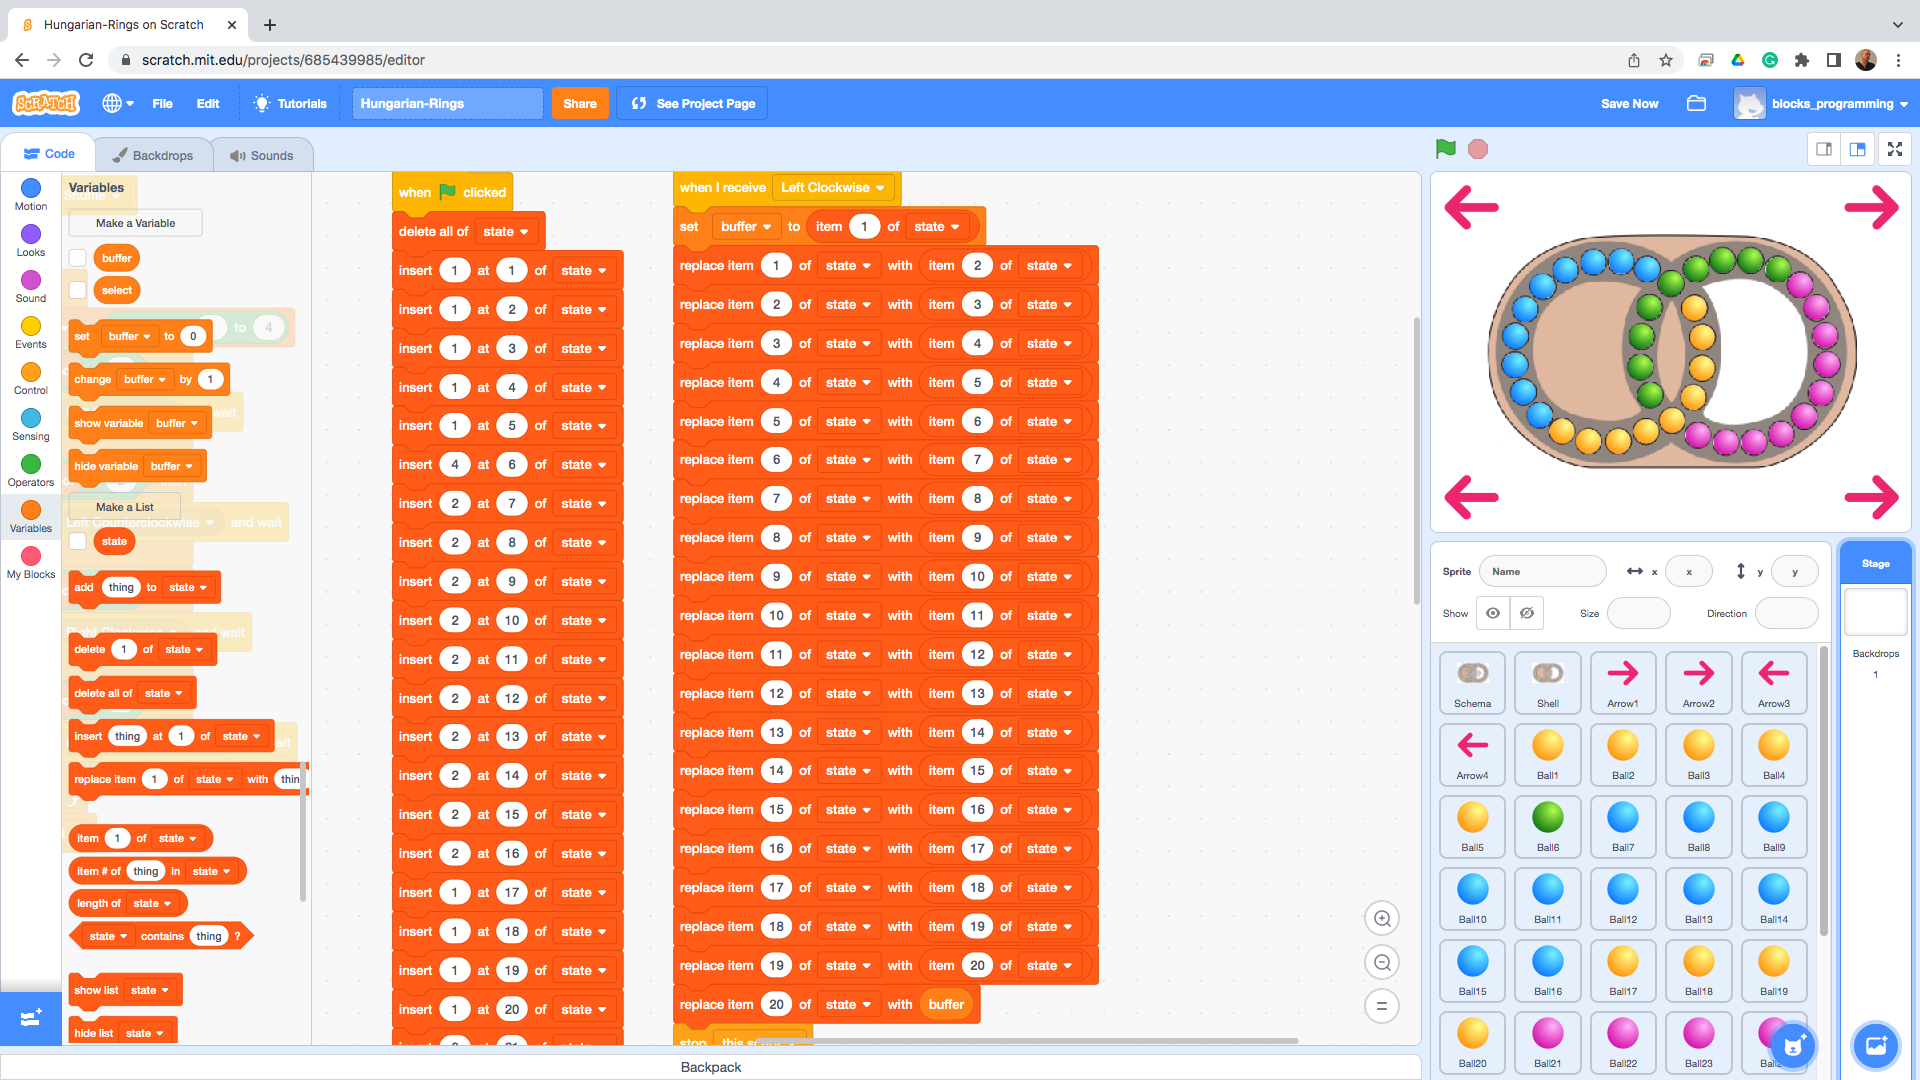
\includegraphics[width=1.0\linewidth,height=0.5\linewidth]{fig050028.png}
  \caption{Инструкции за ротация на левия ринг по часовниковата стрелка}
\label{fig050028}
\end{figure}

Ротацията на левия ринг, обратно на часовниковата стрелка се извършва със следната последователност от действия (Фиг. \ref{fig050029}).

\begin{figure}[H]
  \centering
  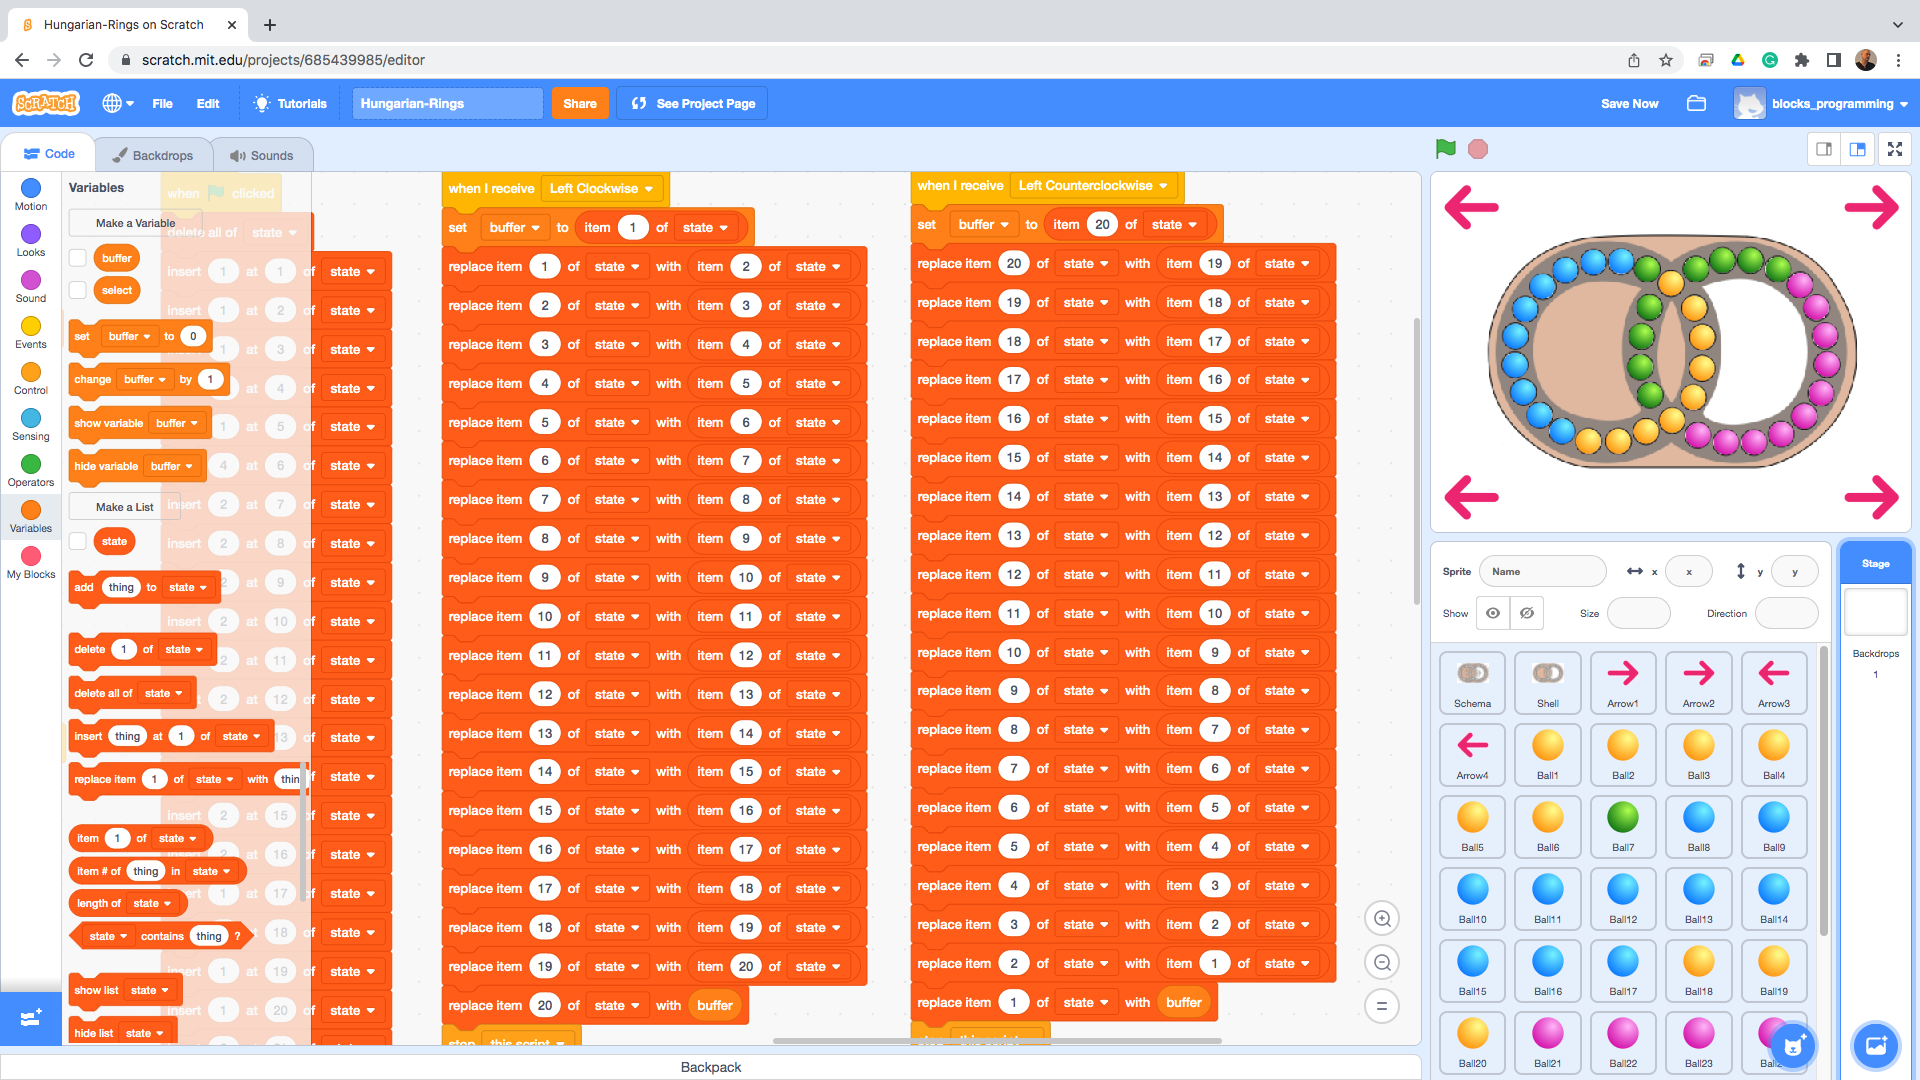
\includegraphics[width=1.0\linewidth,height=0.5\linewidth]{fig050029.png}
  \caption{Инструкции за ротация на левия ринг обратно на часовниковата стрелка}
\label{fig050029}
\end{figure}

Ротацията на десния ринг, по часовниковата стрелка се извършва със следната последователност от действия (Фиг. \ref{fig050030}).

\begin{figure}[H]
  \centering
  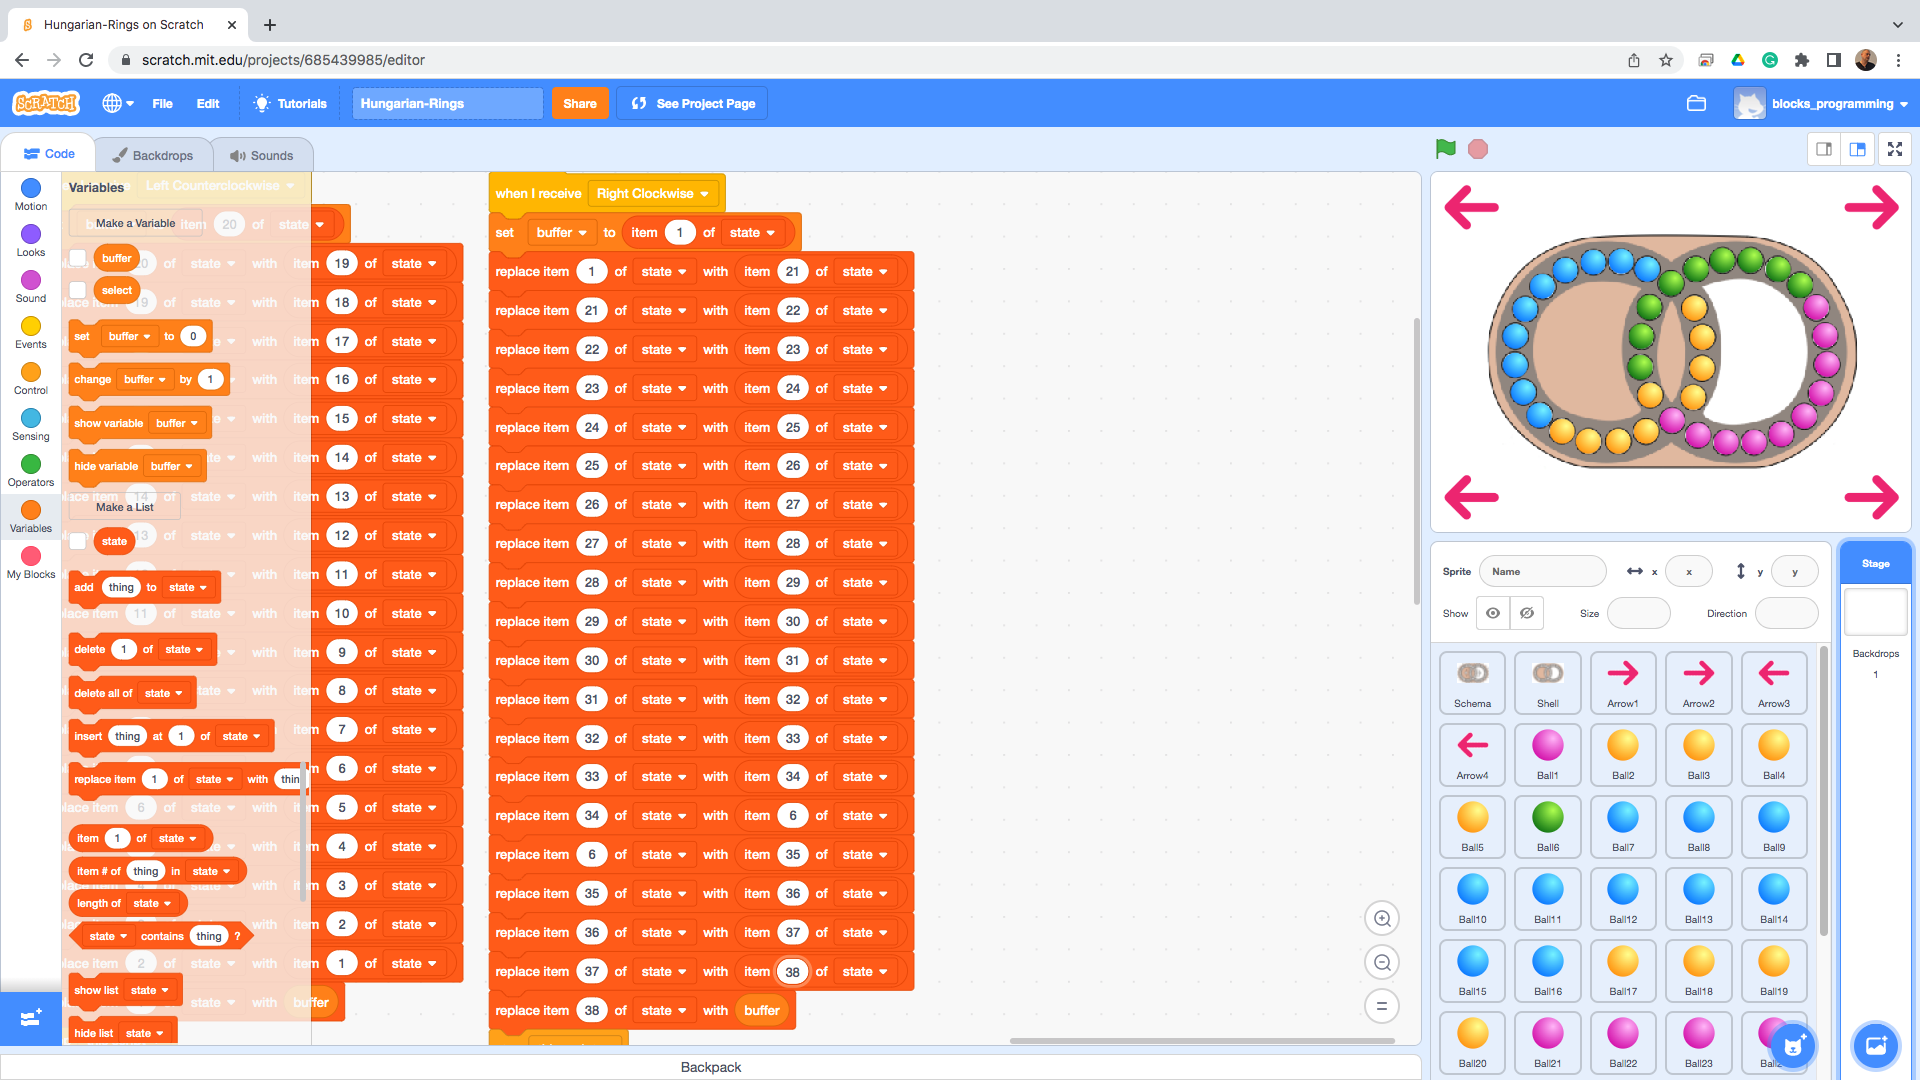
\includegraphics[width=1.0\linewidth,height=0.5\linewidth]{fig050030.png}
  \caption{Инструкции за ротация на десния ринг по часовниковата стрелка}
\label{fig050030}
\end{figure}

Ротацията на десния ринг, обратно на часовниковата стрелка се извършва със следната последователност от действия (Фиг. \ref{fig050031}).

\begin{figure}[H]
  \centering
  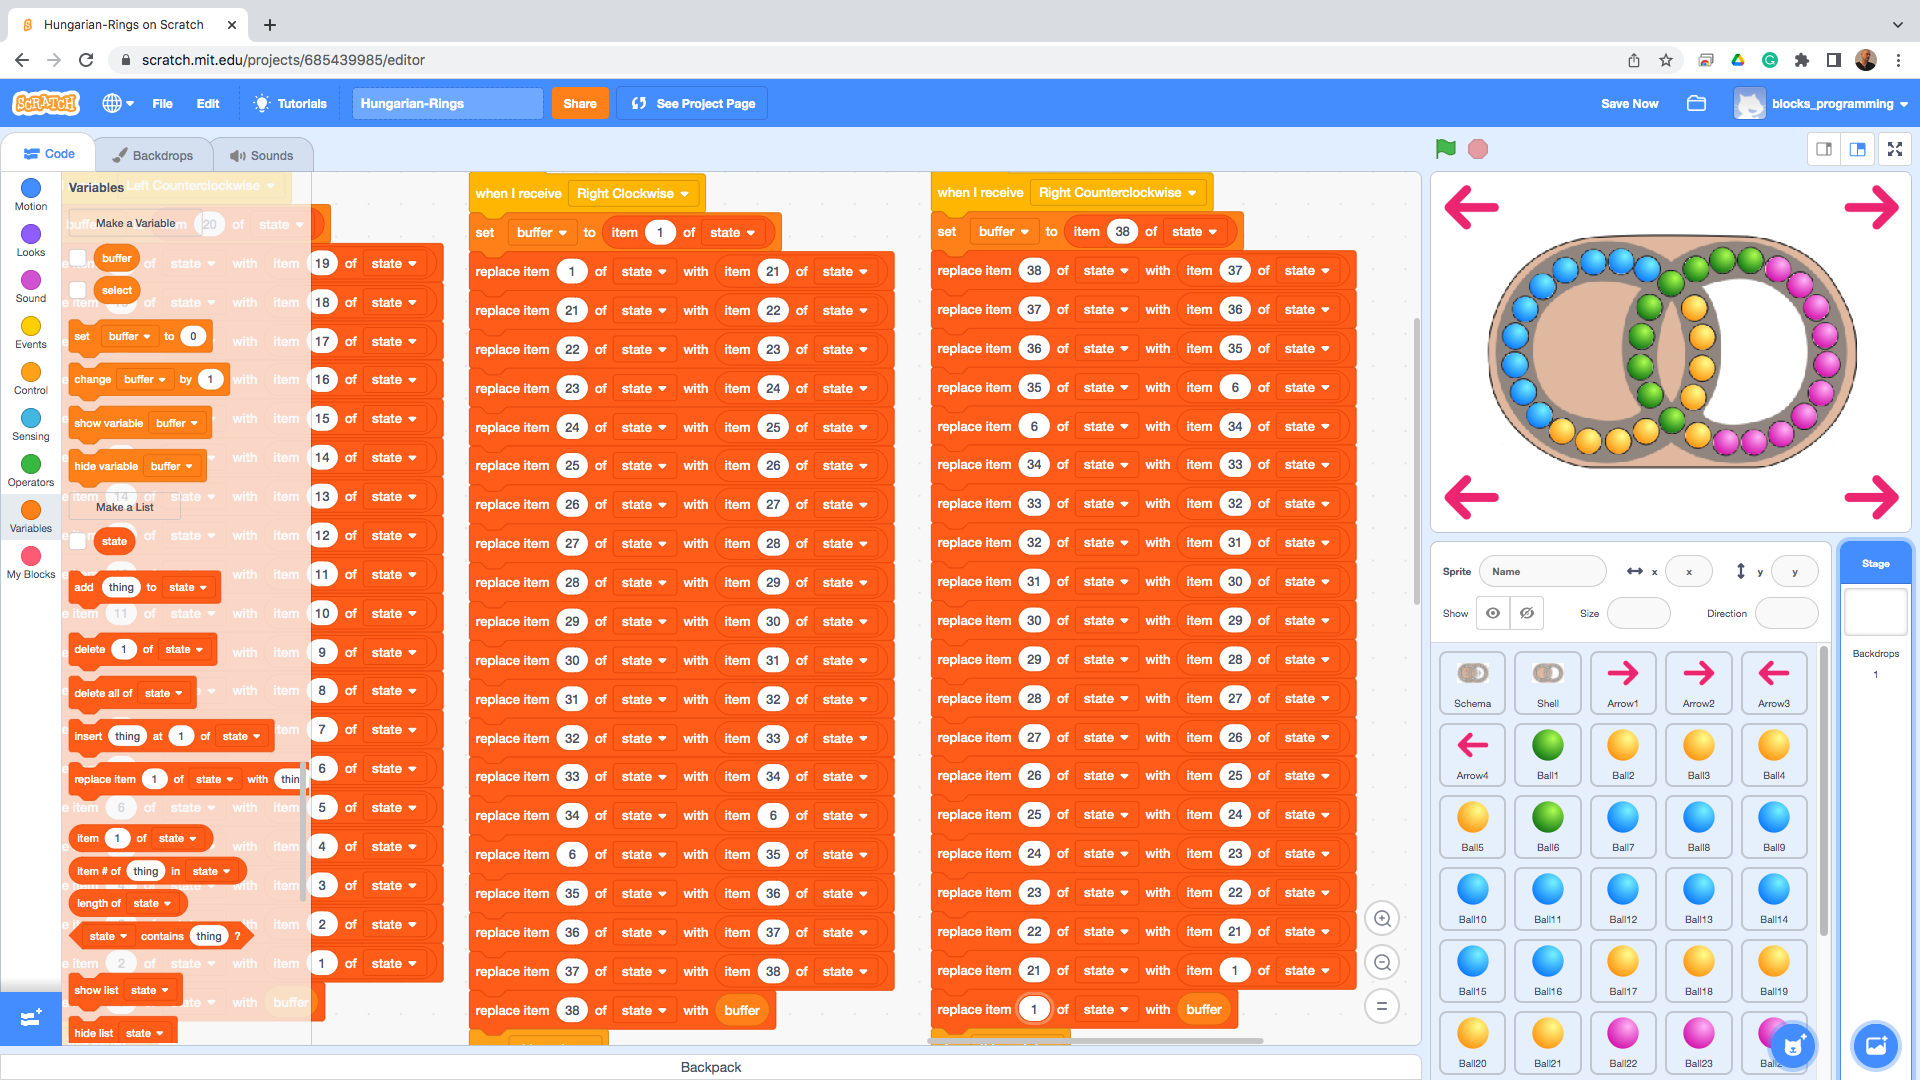
\includegraphics[width=1.0\linewidth,height=0.5\linewidth]{fig050031.png}
  \caption{Инструкции за ротация на десния ринг обратно на часовниковата стрелка}
\label{fig050031}
\end{figure}

\section{Публикуване на проекта}

След изпълнението и на последните инструкции играта придобива своя завършен вид. Разбира се, възможно е да се продължи разработването в посока на алгоритми за нареждане, но тази задача далеч надхвърля възможностите в настоящото изложение. С помощта на бутона „SHARE“ играта бива публикувана за широката аудитория (Фиг. \ref{fig050032}).

\begin{figure}[H]
  \centering
  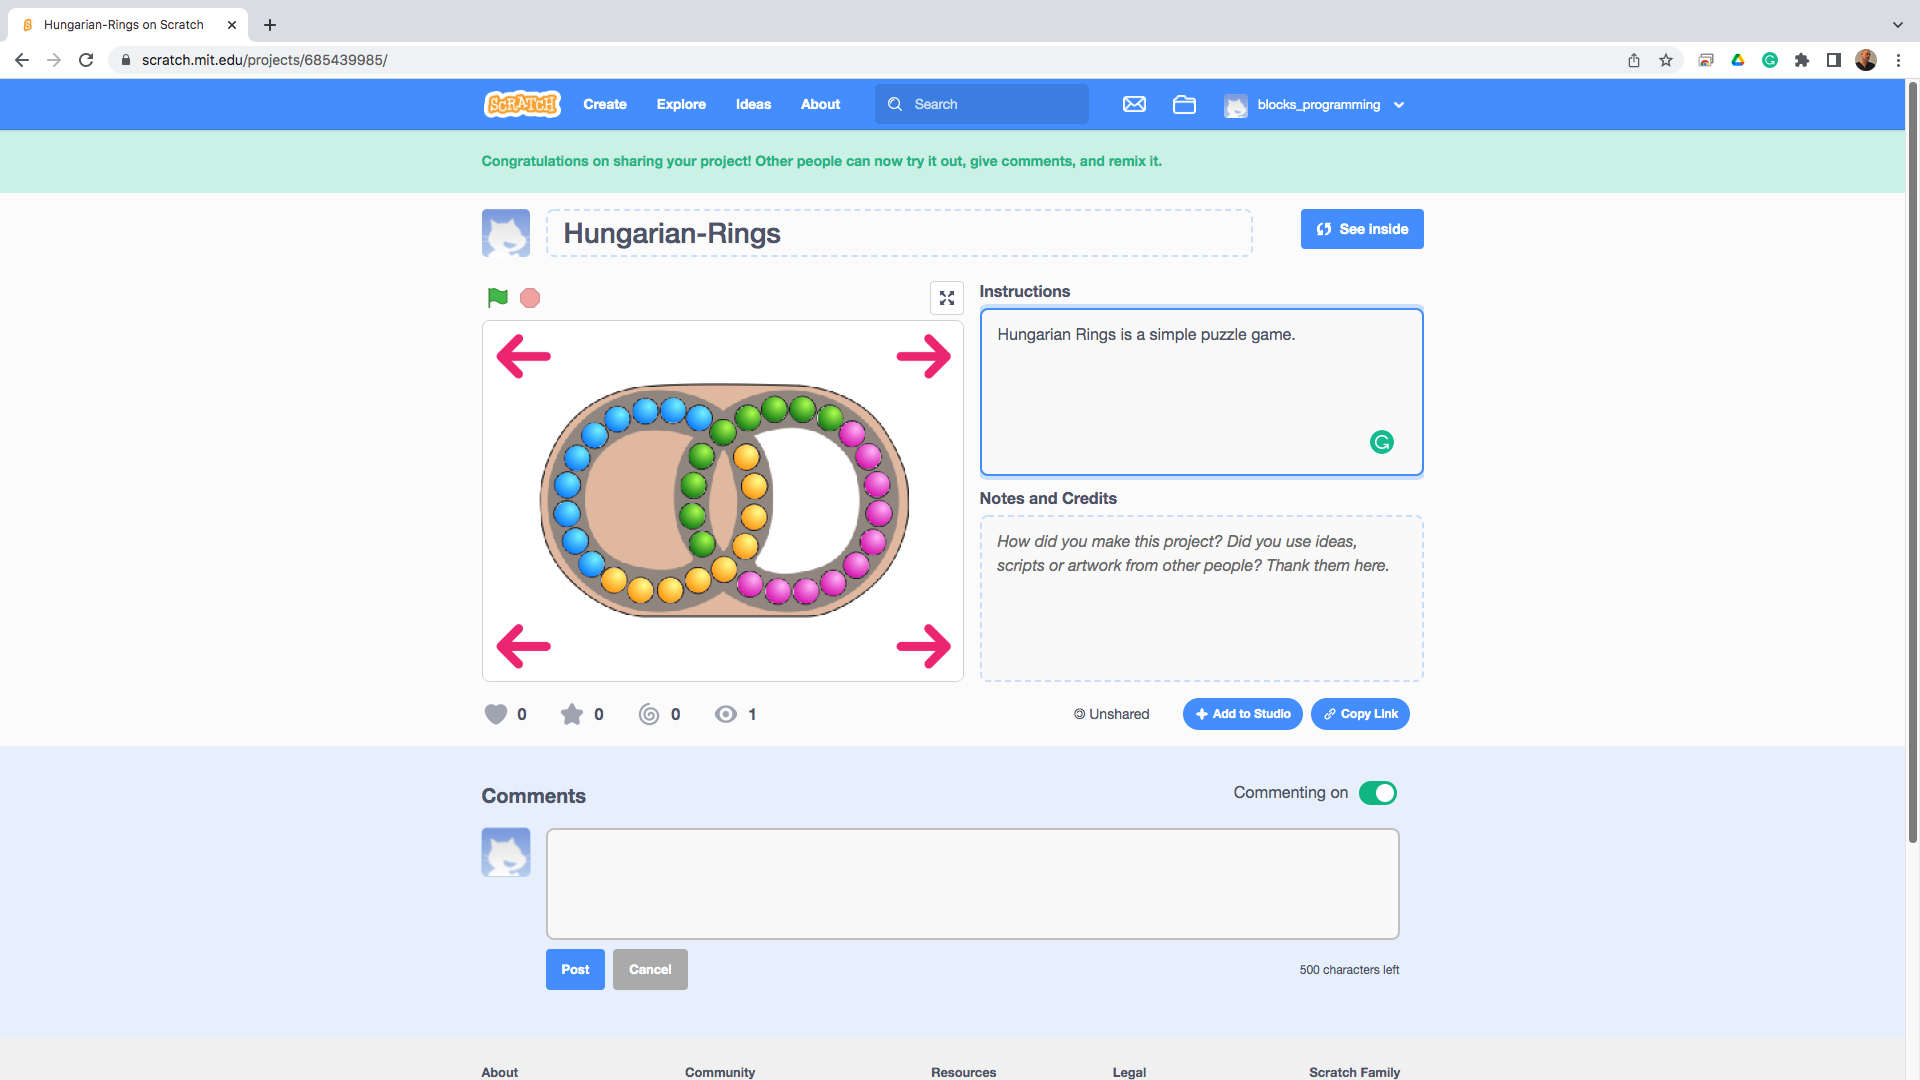
\includegraphics[width=1.0\linewidth,height=0.5\linewidth]{fig050032.png}
  \caption{Споделяне на завършения проект}
\label{fig050032}
\end{figure}

Играта има своя завършен вид, но все още не е оформена като готов, краен продукт. Хубаво би било да се добави функционалност за подреждане на пъзела. Липсва помощна информация. Възможно е да се добави отчитане на времето за подреждане. Всичко изброено носи допълнителна сложност, която е извън обхвата на настоящото изложение, но пък е възможност за допълнително упражнение от страна на читателите.

